\documentclass[a4paper, titlepage]{livret}

\usepackage[utf8]{inputenc}	% accents
\usepackage[T1]{fontenc}	% caractères français
\usepackage{geometry}		% marges
\usepackage[francais]{babel}	% langue
\usepackage{graphicx}		% images
\usepackage{verbatim}		% texte préformaté
\usepackage{listings}		% code source
\usepackage[final]{pdfpages}	% inclusion de pdf
\usepackage{url}		% utilisation des url
\usepackage{caption}		% nom des tableaux
\usepackage{amsmath}		% maths
\usepackage{amsfonts}		% fonts maths
\usepackage[framed,numbered,autolinebreaks,useliterate]{mcode}	% code
\usepackage{titling}
   

\pagestyle{headings}		% rappel discret (en haut à gauche)

\title{Projet de M8}		% titre
\date{}
\author{Elliot Sisteron}	% auteur  

\begin{document} 
\maketitle{}	% page de garde

\setcounter{tocdepth}{1}
\tableofcontents		% table des matières

\chapter*{Introduction}
\addcontentsline{toc}{chapter}{Introduction}	% ajouter l'introduction au sommaire
Depuis toujours, nous avons rencontré la nécessité de protéger certaines informations de la vue d'autrui.
Aujourd'hui où les données s'étalent à n'en plus pouvoir les dénombrer, et où celles-ci représentent parfois des transactions d'une grande importance; 
À l'ère où les géants de l'internet récupèrent des renseignements sur chacun d'entre nous, et où nous comptons plus que tout sur la fiabilité de ces services pour conserver notre vie privée,  il est primordial de mettre l'accent sur la sécurité de nos informations.
C'est pourquoi nous allons nous intéresser dans ce projet aux codes secrets qui ont marqué l'histoire, tant par leur fiabilité apparente au premier abord, que par les conséquences de leur déchiffrement.

Nous nous attarderons dans une première partie sur les chiffres\footnote{Codes secrets} dits de \og substitution \fg{}, qui consistent à remplacer chaque lettre du texte clair par une autre.
Parmi ceux-ci, on choisira les codes de César et de Vigenère, mais aussi un chiffre de substitution mono-alphabétique.
On se proposera surtout d' \og attaquer \fg{} ces chiffres sur des cryptogrammes\footnote{Textes chiffrés}, à l'aide des différents outils que le cours de d'analyse des données nous a fourni.
Nous présenterons tout d'abord rapidement chacun de ces codes.
Puis, nous aurons besoin de faire une analyse statistique sur la langue française et sur les textes à déchiffrer.
Nous verrons ici que cette étude statistique fut à la base même de la cryptanalyse\footnote{Étude du déchiffrement} pendant plus de 1500 ans. 
Nous ferons donc des hypothèses grâce aux données précédemment analysées et nous étudierons la véracité de ces suppositions. 
Si celles-ci s'avèrent cohérentes, nous pourrons enfin les appliquer à la résolution des chiffres et en déduire les textes en clair.

\chapter{Les premiers codes secrets}
\section{Le chiffre de César}
Le chiffre de César doit son nom à l'empereur Jules César qui l'utilisait pour chiffrer ses communications.
Celui-ci consistait en un simple \og décalage \fg{} de l'alphabet :
\begin{center}
  \begin{tabular}{p{1.5cm}*{26}{p{0.1cm}}}
    \hline
    \textbf{Alphabet clair} & a & b & c & d & e & f & g & h & i & j & k & l & m & n & o & p & q & r & s & t & u & v & w & x & y & z \\
    \hline
    \textbf{Alphabet chiffré} & C & D & E & F & G & H & I & J & K & L & M & N & O & P & Q & R & S & T & U & V & W & X & Y & Z & A & B \\
    \hline
  \end{tabular}
   \captionof{table}{Un exemple de décalage César}
  \label{tab1} 
\end{center}

Chaque lettre est substituée à une autre grâce à une clé : un nombre compris entre $1$ et $25$.
Dans l'exemple ci-dessus, la clé est $2$ car l'alphabet chiffré est décalé de deux lettres vers la gauche par rapport à l'alphabet clair. 

Mathématiquement, si l'on numérote les lettres de l'alphabet de $0$ à $25$, et que l'on note :
\begin{itemize}
 \item $x$ la lettre à chiffrer
 \item $y$ la lettre résultante du chiffrement
 \item $c$ la clé comprise entre $1$ et $25$ du chiffre
\end{itemize}
On a la relation suivante :
\[y \equiv x + c \pmod{26} \Leftrightarrow x \equiv y - c \pmod{26}\]

On constate ici qu'un chiffre comme celui-ci peut facilement être brisé en utilisant une \og attaque par force brute \fg{}\footnote{Tentative de \og casser \fg{} le chiffre en essayant toutes les clés possibles} car il n'y a que 25 clés possibles.

\section{Le chiffre de substitution mono-alphabétique}
Ce type de chiffrement fut utilisé pendant longtemps, et le chiffre de César en est un cas particulier.
Son utilisation dura plus d'un millénaire, jusqu'à son déchiffrement au IX siècle par le philosophe arabe Al-Kindi.

\begin{center}
  \begin{tabular}{p{1.5cm}*{26}{p{0.1cm}}}
    \hline
    \textbf{Alphabet clair} & a & b & c & d & e & f & g & h & i & j & k & l & m & n & o & p & q & r & s & t & u & v & w & x & y & z \\
    \hline
    \textbf{Alphabet chiffré} & \textbf{U} & \textbf{N} & \textbf{E} & \textbf{C} & \textbf{L} & A & B & D & F & G & H & I & J & K & M & O & P & Q & R & S & T & V & W & X & Y & Z \\
    \hline
  \end{tabular}
   \captionof{table}{Un exemple de substitution mono-alphabétique}
  \label{tab2} 
\end{center}
  
Là aussi, chaque lettre est substituée à une autre grâce à une clé, mais il s'agit maintenant d'un mot.
Dans notre exemple, le mot utilisé est \og UNECLE \fg{}, le début de l'alphabet chiffré est définit par ce mot-clé, alors que le reste n'est que la suite ordonnée des lettres non-utilisées dans la clé.
La clé peut aussi être un nouvel alphabet (constitué de lettres connues ou bien de signes, libre à l'imagination de celui qui s'improvise cryptographe). 
Ce chiffre est bien plus intéressant que le précédent : il y a $26!$ arrangements de l'alphabet possibles, une \og attaque par force brute \fg{} a donc très peu de chance d'aboutir.
De plus, il est relativement intuitif, pour chiffrer un message on aura tendance à vouloir remplacer une à une chaque lettre du message par une autre.
C'est pour ces raisons qu'il fut omniprésent tout au long de l'histoire, même après son déchiffrement; Ce qui coûta, entre autre, sa vie à Marie Stuart, reine d'Écosse.

\section{Le chiffre de Vigenère}
Ce code secret a vu le jour au XVI siècle, il fut mis en place pour contrer les faiblesses du chiffre mono-alphabétique.
Le chiffre de Vigenère a le bon goût d'être un chiffre poly-alphabétique, c'est-à-dire qu'il utilise plusieurs chiffres mono-alphabétique lors du chiffrement.
En l'occurence, l'idée principale est de \og superposer \fg{} plusieurs alphabets de César à l'aide d'un mot-clé, et de les utiliser un à un à chaque lettre.

\begin{center}
  \begin{tabular}{p{1.5cm}*{26}{p{0.1cm}}}
    \hline
    \textbf{Alphabet clair} & a & b & c & d & e & f & g & h & i & j & k & l & m & n & o & p & q & r & s & t & u & v & w & x & y & z \\
    \hline
    \textbf{Alphabet 1} & \textbf{U} & V & W & X & Y & Z & A & B & C & D & E & F & G & H & I & J & K & L & M & N & O & P & Q & R & S & T \\
    \hline
    \textbf{Alphabet 2} & \textbf{N} & O & P & Q & R & S & T & U & V & W & X & Y & Z & A & B & C & D & E & F & G & H & I & J & K & L & M \\
    \hline
    \textbf{Alphabet 3} & \textbf{E} & F & G & H & I & J & K & L & M & N & O & P & Q & R & S & T & U & V & W & X & Y & Z & A & B & C & D \\
    \hline
    \textbf{Alphabet 4} & \textbf{C} & D & E & F & G & H & I & J & K & L & M & N & O & P & Q & R & S & T & U & V & W & X & Y & Z & A & B \\
    \hline
    \textbf{Alphabet 5} & \textbf{L} & M & N & O & P & Q & R & S & T & U & V & W & X & Y & Z & A & B & C & D & E & F & G & H & I & J & K \\
    \hline
    \textbf{Alphabet 6} & \textbf{E} & F & G & H & I & J & K & L & M & N & O & P & Q & R & S & T & U & V & W & X & Y & Z & A & B & C & D \\
    \hline
  \end{tabular}
   \captionof{table}{Un exemple de chiffrement Vigenère}
  \label{tab3} 
\end{center}

La taille du mot-clé définit le nombre d'alphabets que l'on utilisera.
Les lettres qui forment le mot-clé définissent quant à elles les alphabets de César utilisés dans le chiffrement.
Ici, la clé utilisée est aussi \og UNECLE \fg{}.
Dans cet exemple, pour chiffrer un message, il suffit de chiffrer la première lettre avec l'alphabet $1$, la deuxième avec l'alphabet $2$, …, la septième avec l'alphabet $1$, etc.
Si l'on note $k$ la taille du mot-clé, on a donc $26^k$ chiffres possibles.
Il a été prouvé mathématiquement que ce chiffre est \og \emph{incassable} \fg{} sous certaines conditions : la clé doit être de la taille du message à chiffrer, unique, et elle se doit aussi d'être générée aléatoirement.
Pour des raisons pratiques, on ne l'utilise pas aujourd'hui : la taille de la clé deviendrait trop importante et, surtout, il est impossible de reproduire un phénomène purement aléatoire informatiquement (ce genre de phénomène n'existant que dans la nature).
\newpage
\section{Les cryptogrammes à déchiffrer dans ce projet}

On essaiera dans ce projet de déchiffrer les cryptogrammes suivants :

\begin{itemize}

\item Cryptogramme n\textdegree1 :
\begin{center}
\begin{quote}
\og FILMK OYFYP CHYHN LYFYM YWLYN MILNF YNUFG OX \fg{}
\end{quote}
\end{center}

\item Cryptogramme n\textdegree2 :
\begin{center}
\begin{quote}
\og JHCKG TDWNF WAXXV WQKWA GIIKE NQDMT QLRXJ GBGMG IW-
MEO NDSWL MKWMC SHBWF AHQKW CMVCB AJSLC ESKUS JBMSI
CWMFW PMWTD WQOWM GCMVW KIAGJ CWQXA LRTJG FWLWG
KMFQH VLFXA VSLOW BLYMW FWFHM MFRNT SATQF DXCLS MZ-
WON VECFM FHHCB SGMHC NDSWL XSGHC BSMIA GLMMZ VPWNF
WASMK WGMKM FBMML WMKSW QJSJC WZXAZ OLIJR LTWGK MF-
QHV LFXAX CKOWB MCFSW MKHBV WSIIJ QXYMS JCSBW WFOEM
YCNBV SEIUV HAWEN IFRHV SZXOG IMLWZ TKZCL MTWXV XOBBW
ZXJWO NOWGM MHOKN GWLWF BXBJC NDWDT ADWGB WFEWU
IMMMF XVXOV MBSWQ JOBAD SFQJC BZIIB DGILI ARXIS JTVUS KIDCK
AUSGM KHIIK AHVUO LKGAF MBSWQ KOBAD OICAG JCWAH QSIVW
FHKIA FXRSW ICWHC MVWLU WFVQS ZTDAS CMDIB LAGFM JQBRW
QAIFH XTSJB MBSWI FGXTS JBMBS GMKIB AIITU GIKML TBVSZ XUWBM
YMOGL TSTCU CNXVS ZMFGF MVWLM FHFIA GVWEA XVLTT QKHNX
GIKIN CBZUS MBWVN USBBB WXXTW IKZWD HVVGM ZWGLQ EDEME
SGBBS EMMFW QKENM USLBU SZWMH WMDOF WMFJC AATXG ILAWO
NRGIK LZIBI WBMZW DKMFR KMMBX KGBLB JIVBA CGUWQ TVAEN
MEOBA VSFIA BJCAG TQLDX CLSMZ WGXCD SFMFH TUWAX BLFXI
MGXZN WVMVS EIUCF UMBTC LSTNS WKMDS WWFZX LGBWM KCB \fg{}
\end{quote}
\end{center}

\item Cryptogramme n\textdegree3 :
\begin{center}
\begin{quote}
\og OHQSB SAQSA MTOQF BFJAN OQLPB HNQHJ GEPOQ OHBHL FBAQF BWJUF BPLOH TGEOP QBEPL FFHOX KPAGO FOUBA SMTOF OQRBP BRSPA QSAMT OQNTH RIBHS AFFJH BFBSJ APOQO PBKKP JRIOH SNBTS BHSKF TQNOQ RBPBR SPAQS AMTOQ QSBSA QSAMT OQNOF BKJKT FBSAJ HMTOF BSBAF FONOF RIBHS AFFJH BTLGO HSOFB SBAFF ONOFR IBHSA FFJHR JHQAN POPKJ TPBKK PJRIO PFOQR BPBRS PAQSA MTOQN OFBKJ KTFBS AJHHO NKOHN MTOUB AEFOG OHSVJ APOKB QNTSJ TSNOF BSBAF FONOR OFFOR AMTOF OQJHN BLOQJ ASUBA SBTFT XOGEJ TPLJT BTXSB SQTHA QAFQT UUASK JTPJE SOHAP NOQKP RAQAJ HQLBF OQNOK POHNP ONOQR IBHSA FFJHQ NOSBA FFOQL BFOQ \fg{}
\end{quote}
\end{center}

\end{itemize}

\chapter{Calcul des fréquences}
Dans cette partie nous étudierons des données sur l'utilisation des lettres de l'alphabet et des bigrammes dans la langue française et dans les textes à déchiffrer.
On calculera en particulier les \emph{indices de coïncidence} de chaque cryptogramme, pour savoir par quel cryptosystème\footnote{Mécanisme de chiffrement et de déchiffrement} est chiffré chaque texte.
Nous nous intéresserons aussi aux mots les plus fréquents, car ceux-là auront une forte probabilité d'apparaître dans les cryptogrammes.
On se propose de récupérer ces données, pour ensuite essayer de les représenter.

\section{Génération des données}
Nous essayons d'avoir une estimation correcte de la fréquence d'utilisation de chaque lettre de l'alphabet en français.
Pour cela, il est nécessaire de choisir un ou plusieurs textes sur lesquels on utilisera un script\footnote{Ce script est disponible en annexe} de calcul des effectifs de chaque lettre.
Ici, nous avons choisi les \oe{}uvres suivantes :
\begin{itemize}
\item \emph{La fille aux yeux d'or}, \textsc{Honoré de Balzac}
\item \emph{Les antiquités de Rome}, \textsc{Joachim du Bellay}
\item \emph{Madame Bovary}, \textsc{Gustave Flaubert}
\item \emph{Notre dame de Paris}, \textsc{Victor Hugo}
\item \emph{La science et l'hypothèse}, \textsc{Henri Poincaré}
\item \emph{Gargantua}, \textsc{François Rabelais}
\item \emph{Le tour du monde en quatre-vingt jours}, \textsc{Jules Verne}
\item \emph{Candide}, \textsc{Voltaire}
\item \emph{Germinal}, \textsc{Émile Zola}
\end{itemize} 
Étant donné que les caractères spéciaux (é, è, à…) sont remplacés par leurs parents lors du chiffrement, le \og é \fg{} compte donc pour un \og e \fg{}, le \og à \fg{} pour un \og a \fg{}, etc.

De plus, nous recherchons aussi la fréquence de chaque bigramme dans la langue française. 
Pour ce faire, nous appliquons un autre script\footnote{Disponible en annexe} sur les textes énumérés précédemment.

Enfin, pour pouvoir \og casser \fg{} des codes César et mono-alphabétique, nous aurons besoin de calculer, de même, la fréquence de chaque lettre, chaque bigramme des textes (en utilisant les scripts précédents).
Pour ce qui est d'un chiffre de Vigenère, il faut faire la supposition que le mot-clé ne dépasse pas les $k$ lettres.
Autrement dit, il sera nécessaire de trouver le naturel $k$ qui est statistiquement le plus plausible.
Il est inutile pour un tel chiffre d'étudier les bigrammes car celui-ci est poly-alphabétique : ces fréquences n'auraient pas de sens.

\section{Indice de coïncidence}
Étant donné que nous ne savons pas quel code est appliqué sur chaque cryptogramme, il nous est nécessaire d'avoir un outil nous permettant d'avoir une idée du chiffre utilisé.
L'indice de coïncidence d'un texte permet de savoir si chaque lettre est uniformément distribuée ou non, ce qui permet d'en déduire la nature mono-alphabétique ou poly-alphabétique du texte étudié.
Cet outil a été inventé par William F. Friedman en $1920$, et c'est pour cette raison qu'on appelle le test appliqué sur les cryptogrammes le test de Friedman.
L'indice de coïncidence est défini par la formule suivante : 
\[ IC = \sum_{l = A}^{Z} \frac{n_{l}(n_{l} - 1)}{n(n-1)} \]
avec :
\begin{itemize}
 \item $IC$ l'indice de coïncidence
 \item $n_{l}$ les effectifs de la lettre $l$ dans le texte
 \item $n$ le nombre total de lettres dans le texte
\end{itemize}

En fait, si on pose $E_{l}$ l'événement \og La lettre $l$ apparaît deux fois de suite dans le tirage sans remise de deux lettres au hasard dans le texte \fg{} on peut dire ici que :
\[ IC = \sum_{l = A}^{Z} \mathbb{P}(E_{l}) \]
Il s'agit donc ici de la probabilité d'obtenir une paire de lettres quelconques en tirant deux lettres dans le texte étudié.

\section{Description des données}
Les scripts précédents nous ont permis d'obtenir les effectifs de chaque lettre/bigramme dans un fichier donné.
Toutefois, pour se faire une idée de l'utilisation de chaque élément, il nous est nécessaire de calculer la fréquence d'apparition de ceux-ci.
De plus, on aimerait pouvoir se représenter ces données avec des histogrammes.
Pour cela, on traite les données des scripts avec MatLab\footnote{Le code source de ce traitement MatLab est disponible en annexe}.

\subsection{Fréquence de chaque lettre en français}

\begin{minipage}[c]{.3\linewidth}
  \begin{tabular}{|c|c|c|}
    \hline
	 & \textbf{Nb} & \textbf{\%}\\
	 \hline
    	\textbf{A} &  279823 &  8.59\\
	\hline
	\textbf{B} &   33102 &  1.02\\
	\hline
	\textbf{C} &  100170 &  3.08\\
	\hline
	\textbf{D} &  120611 &  3.70\\
	\hline
	\textbf{E} &  557202 &  17.11\\
	\hline
	\textbf{F} &   35930 &  1.10\\
	\hline
	\textbf{G} &   34934 &  1.07\\
	\hline
	\textbf{H} &   32630 &  1.00\\
	\hline
	\textbf{I} &  239698 &  7.36\\
	\hline
	\textbf{J} &   13668 &  0.42\\
	\hline
	\textbf{K} &     508 &  0.02\\
	\hline
	\textbf{L} &  192759 &  5.92\\
	\hline
	\textbf{M} &   90806 &  2.79\\
	\hline
	\textbf{N} &  225182 &  6.91\\
	\hline
	\textbf{O} &  173499 &  5.33\\
	\hline
	\textbf{P} &   88040 &  2.70\\
	\hline
	\textbf{Q} &   38380 &  1.18\\
	\hline
	\textbf{R} &  213830 &  6.57\\
	\hline
	\textbf{S} &  257287 &  7.90\\
	\hline
	\textbf{T} &  238266 &  7.32\\
	\hline
	\textbf{U} &  207131 &  6.36\\
	\hline
	\textbf{V} &   51963 &  1.60\\
	\hline
	\textbf{W} &     348 &  0.01\\
	\hline
	\textbf{X} &   13849 &  0.43\\
	\hline
	\textbf{Y} &   11602 &  0.36\\
	\hline
	\textbf{Z} &    5614 &  0.17\\
	\hline
	\textbf{Total} &  3256832 &  100.00\\
	\hline
  \end{tabular}
   \captionof{table}{Résultat des calculs de fréquences}
  \label{tab4}
\end{minipage}
\begin{minipage}[c]{.9\linewidth}
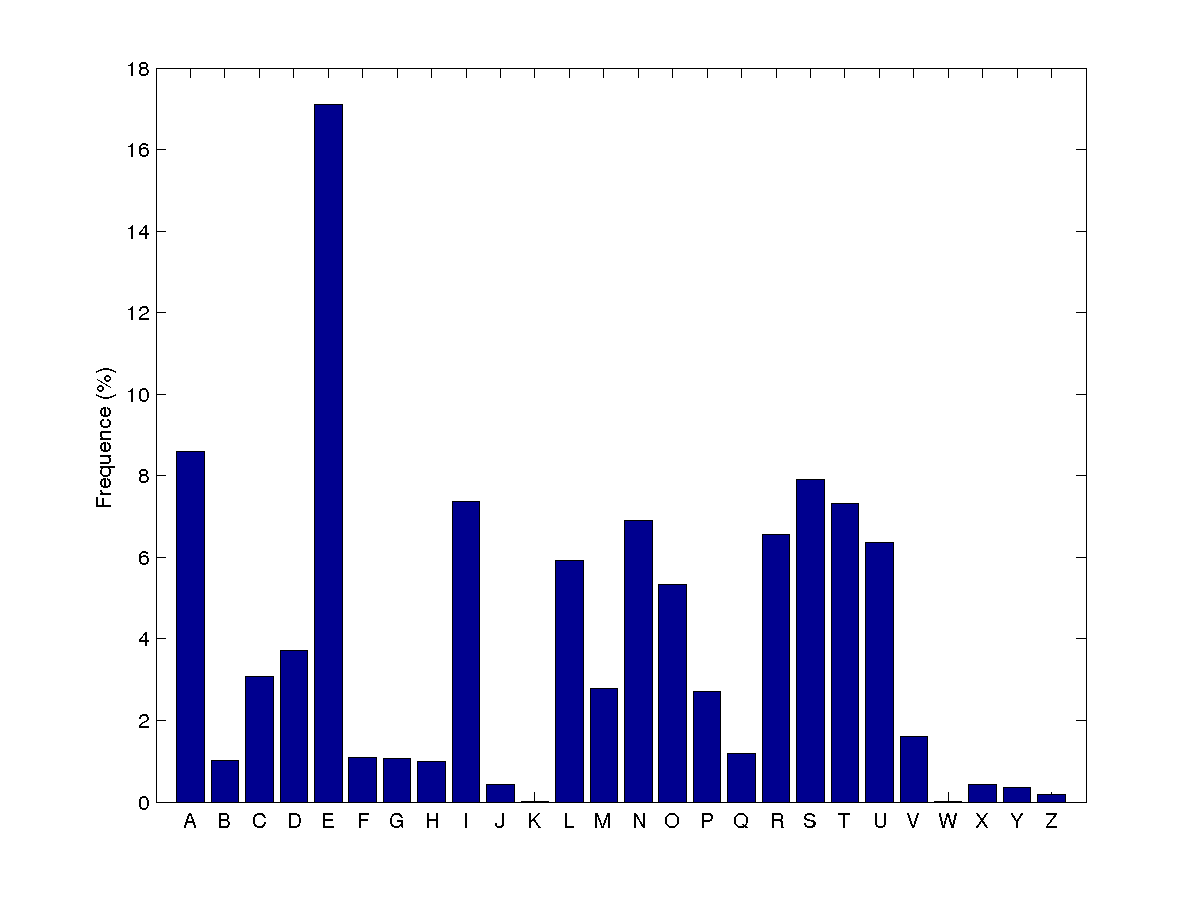
\includegraphics[width=13cm]{img/LettreFreqTexte.png}
\captionof{figure}{Visualisation des fréquences de chaque lettre}
\label{fig1}
\end{minipage}

\begin{center}
\begin{tabular}{|c|c|c|}
	\hline
	& \textbf{Effectifs} & \textbf{Fréquences}\\
	\hline
	\textbf{Moyenne} &  125263 &  3.85\\
	\hline
	\textbf{Variance} &  16711876115 &  15.76\\
	\hline
	\textbf{Écart-type} &  129274 &  3.97\\
	\hline
	\textbf{Médiane} &  89423 &  2.75\\
	\hline
\end{tabular}
\label{tab5}
\captionof{table}{Description des variables}
\end{center}

\begin{center}
\begin{tabular}{|c|}
\hline
\textbf{$IC = 0,0779$}\\
\hline
\end{tabular}
\label{tab6}
\captionof{table}{Indice de coïncidence}
\end{center}

Cet indice de coïncidence correspond, à $10^{-4}$ près, à celui que l'on retrouve sur \emph{Wikipédia}, on peut donc en déduire que les données générées sont très représentatives de la langue française.
On fera donc l'approximation que les fréquences que l'on a calculées sont les probabilités réelles de chaque lettre.

\subsection{Fréquence de chaque bigramme en français}
Ici, on ne montrera que les $26$ bigrammes les plus fréquents en français (les autres ne nous seront pas utiles).
De plus, on s'intéresse aussi à la fréquence de chaque paire de lettres.\\

\begin{center}
\begin{minipage}[c]{.3\linewidth}
\begin{tabular}{|c|c|c|}
 \hline
	& \textbf{Nb} & \textbf{(\%)}\\
	\hline
 	\textbf{LE} &   12124 &  1.19\\
	\hline
	\textbf{EN} &   11990 &  1.18\\
	\hline
	\textbf{RE} &   11730 &  1.15\\
	\hline
	\textbf{OU} &   11326 &  1.11\\
	\hline
	\textbf{ON} &   11315 &  1.11\\
	\hline
	\textbf{IT} &   11076 &  1.09\\
	\hline
	\textbf{ES} &   11034 &  1.09\\
	\hline
	\textbf{NT} &   10973 &  1.08\\
	\hline
	\textbf{AI} &   10924 &  1.07\\
	\hline
	\textbf{DE} &   10907 &  1.07\\
	\hline
	\textbf{QU} &   10319 &  1.02\\
	\hline
	\textbf{AN} &   10218 &  1.01\\
	\hline
	\textbf{UR} &    9756 &  0.96\\
	\hline
	\textbf{ER} &    9724 &  0.96\\
	\hline
	\textbf{TE} &    9664 &  0.95\\
	\hline
	\textbf{LA} &    9473 &  0.93\\
	\hline
	\textbf{IS} &    9408 &  0.93\\
	\hline
	\textbf{IL} &    9227 &  0.91\\
	\hline
	\textbf{NE} &    9195 &  0.90\\
	\hline
	\textbf{SE} &    9150 &  0.90\\
	\hline
	\textbf{ME} &    9141 &  0.90\\
	\hline
	\textbf{IE} &    9100 &  0.90\\
	\hline
	\textbf{EU} &    9096 &  0.90\\
	\hline
	\textbf{IN} &    8865 &  0.87\\
	\hline
	\textbf{AR} &    8734 &  0.86\\
	\hline
	\textbf{PA} &    8454 &  0.83\\
	\hline
\end{tabular}
   \captionof{table}{Fréquences sur les bigrammes}
  \label{tab19}
\end{minipage}
\begin{minipage}[c]{.3\linewidth}
 \begin{tabular}{|c|c|c|}
 \hline
	& \textbf{Nb} & \textbf{(\%)}\\
	\hline
	\textbf{AA} &      10 &  0.00\\
	\hline
	\textbf{BB} &     122 &  0.01\\
	\hline
	\textbf{CC} &    1359 &  0.13\\
	\hline
	\textbf{DD} &      28 &  0.00\\
	\hline
	\textbf{EE} &      66 &  0.01\\
	\hline
	\textbf{FF} &    2588 &  0.25\\
	\hline
	\textbf{GG} &     631 &  0.06\\
	\hline
	\textbf{HH} &       6 &  0.00\\
	\hline
	\textbf{II} &     184 &  0.02\\
	\hline
	\textbf{JJ} &       0 &  0.00\\
	\hline
	\textbf{KK} &       0 &  0.00\\
	\hline
	\textbf{LL} &    7771 &  0.76\\
	\hline
	\textbf{MM} &    5063 &  0.50\\
	\hline
	\textbf{NN} &    4413 &  0.43\\
	\hline
	\textbf{OO} &     103 &  0.01\\
	\hline
	\textbf{PP} &    2360 &  0.23\\
	\hline
	\textbf{QQ} &       0 &  0.00\\
	\hline
	\textbf{RR} &    3954 &  0.39\\
	\hline
	\textbf{SS} &    6746 &  0.66\\
	\hline
	\textbf{TT} &    4349 &  0.43\\
	\hline
	\textbf{UU} &       2 &  0.00\\
	\hline
	\textbf{VV} &       0 &  0.00\\
	\hline
	\textbf{WW} &       0 &  0.00\\
	\hline
	\textbf{XX} &      60 &  0.01\\
	\hline
	\textbf{YY} &       0 &  0.00\\
	\hline
	\textbf{ZZ} &       0 &  0.00\\
	\hline
\end{tabular}
   \captionof{table}{Fréquences sur les paires}
  \label{tab20}
\end{minipage}
\end{center}

\begin{center}
\begin{tabular}{|c|c|c|}
	\hline
	& \textbf{Effectifs} & \textbf{Fréquences}\\
	\hline
	\textbf{Moyenne} &  1503 &  0.15\\
	\hline
	\textbf{Variance} &  7169716 &  0.07\\
	\hline
	\textbf{Écart-type} &  2678 &  0.26\\
	\hline
	\textbf{Médiane} &   46 &  0.00\\
	\hline
\end{tabular}
\label{tab12}
\captionof{table}{Description des variables}
\end{center}

On se restreint à étudier les bigrammes sur un texte plus petit (environ 1 million de bigrammes), car le script bash ne fonctionne pas autrement.
Les fréquences sont donc un peu moins précises, mais rien d'affolant.
On fera, là aussi, l'approximation que les fréquences calculées correspondent à la probabilité d'apparition de chaque bigramme.


\subsection{Fréquence de chaque lettre dans les cryptogrammes}

\subsubsection{Pour le cryptogramme n\textdegree1}

\begin{minipage}[c]{.3\linewidth}
  \begin{tabular}{|c|c|c|}
    \hline
	& \textbf{Nb} & \textbf{\%}\\
	 \hline
	\textbf{A} &       0 &  0.00\\
	\hline
	\textbf{B} &       0 &  0.00\\
	\hline
	\textbf{C} &       1 &  2.70\\
	\hline
	\textbf{D} &       0 &  0.00\\
	\hline
	\textbf{E} &       0 &  0.00\\
	\hline
	\textbf{F} &       5 &  13.51\\
	\hline
	\textbf{G} &       1 &  2.70\\
	\hline
	\textbf{H} &       2 &  5.41\\
	\hline
	\textbf{I} &       2 &  5.41\\
	\hline
	\textbf{J} &       0 &  0.00\\
	\hline
	\textbf{K} &       1 &  2.70\\
	\hline
	\textbf{L} &       4 &  10.81\\
	\hline
	\textbf{M} &       3 &  8.11\\
	\hline
	\textbf{N} &       4 &  10.81\\
	\hline
	\textbf{O} &       2 &  5.41\\
	\hline
	\textbf{P} &       1 &  2.70\\
	\hline
	\textbf{Q} &       0 &  0.00\\
	\hline
	\textbf{R} &       0 &  0.00\\
	\hline
	\textbf{S} &       0 &  0.00\\
	\hline
	\textbf{T} &       0 &  0.00\\
	\hline
	\textbf{U} &       1 &  2.70\\
	\hline
	\textbf{V} &       0 &  0.00\\
	\hline
	\textbf{W} &       1 &  2.70\\
	\hline
	\textbf{X} &       1 &  2.70\\
	\hline
	\textbf{Y} &       8 &  21.62\\
	\hline
	\textbf{Z} &       0 &  0.00\\
	\hline
	\textbf{Total} &      37 &  100.00\\
	\hline
  \end{tabular}
   \captionof{table}{Résultat des calculs de fréquences}
  \label{tab8}
  \end{minipage} \hfill
\begin{minipage}[c]{.85\linewidth}\centering
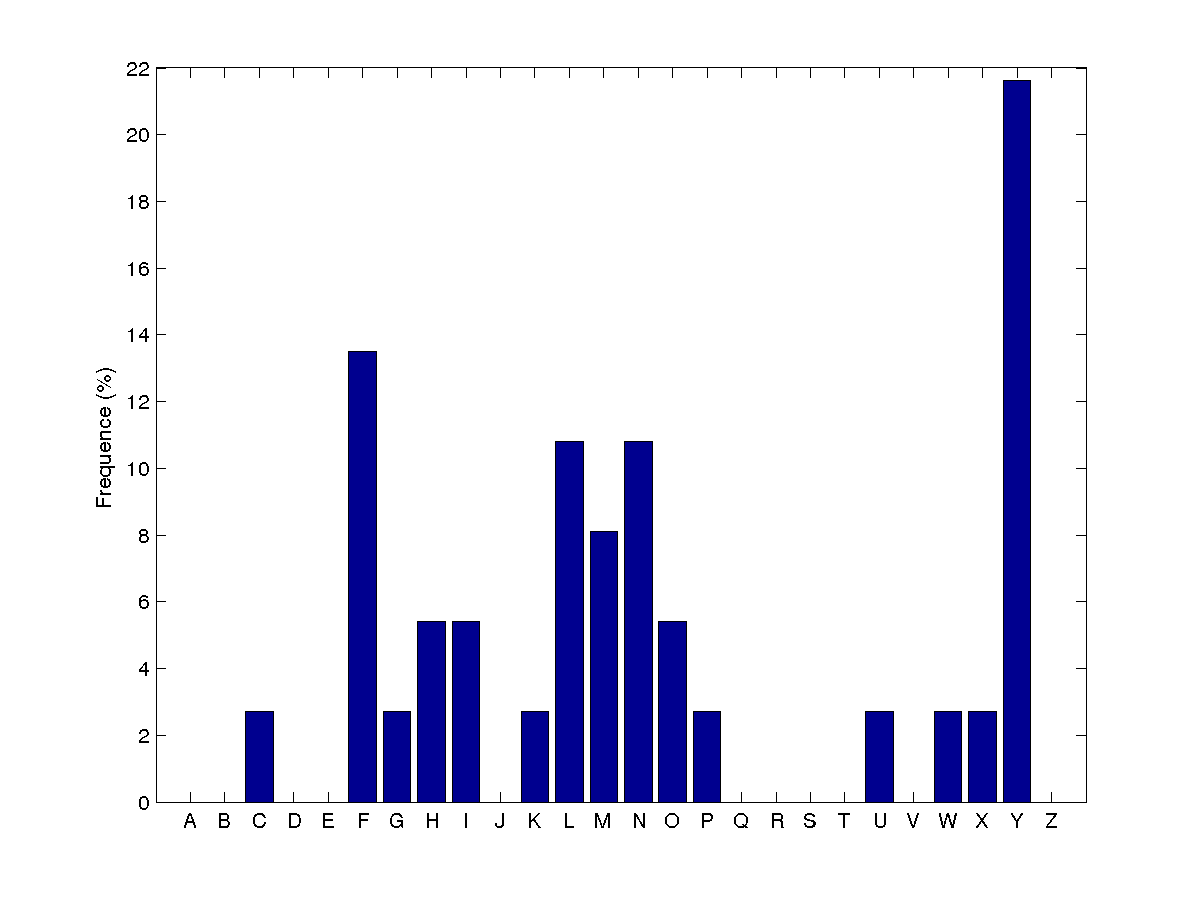
\includegraphics[width=13cm]{img/LettreFreqCesar.png}
\captionof{figure}{Visualisation des fréquences de chaque lettre}
\label{fig2}
\end{minipage} \hfill

\begin{center}
\begin{tabular}{|c|c|c|}
	\hline
	& \textbf{Effectifs} & \textbf{Fréquences}\\
	\hline
	\textbf{Moyenne} &    1.42 &  3.85\\
	\hline
	\textbf{Variance} &    3.85 &  28.15\\
	\hline
	\textbf{Écart-type} &    1.96 &  5.31\\
	\hline
	\textbf{Médiane} &    1.00 &  2.70\\
	\hline
\end{tabular}
\label{tab9}
\captionof{table}{Description des variables}
\end{center}

\begin{center}
\begin{tabular}{|c|}
\hline
\textbf{$IC = 0.0841$}\\
\hline
\end{tabular}
\label{tab10}
\captionof{table}{Indice de coïncidence}
\end{center}

Avec un $IC$ aussi proche du français, on peut faire l'hypothèse que ce cryptogramme résulte d'un chiffrement mono-alphabétique.

\subsubsection{Pour le cryptogramme n\textdegree2}

\begin{minipage}[c]{.3\linewidth}
  \begin{tabular}{|c|c|c|}
    \hline
	& \textbf{Nb} & \textbf{\%}\\
	\hline
		\textbf{A} &      38 &  4.53\\
	\hline
	\textbf{B} &      52 &  6.21\\
	\hline
	\textbf{C} &      38 &  4.53\\
	\hline
	\textbf{D} &      22 &  2.63\\
	\hline
	\textbf{E} &      17 &  2.03\\
	\hline
	\textbf{F} &      44 &  5.25\\
	\hline
	\textbf{G} &      41 &  4.89\\
	\hline
	\textbf{H} &      25 &  2.98\\
	\hline
	\textbf{I} &      44 &  5.25\\
	\hline
	\textbf{J} &      23 &  2.74\\
	\hline
	\textbf{K} &      35 &  4.18\\
	\hline
	\textbf{L} &      36 &  4.30\\
	\hline
	\textbf{M} &      75 &  8.95\\
	\hline
	\textbf{N} &      21 &  2.51\\
	\hline
	\textbf{O} &      21 &  2.51\\
	\hline
	\textbf{P} &       2 &  0.24\\
	\hline
	\textbf{Q} &      23 &  2.74\\
	\hline
	\textbf{R} &      10 &  1.19\\
	\hline
	\textbf{S} &      52 &  6.21\\
	\hline
	\textbf{T} &      27 &  3.22\\
	\hline
	\textbf{U} &      18 &  2.15\\
	\hline
	\textbf{V} &      33 &  3.94\\
	\hline
	\textbf{W} &      80 &  9.55\\
	\hline
	\textbf{X} &      36 &  4.30\\
	\hline
	\textbf{Y} &       4 &  0.48\\
	\hline
	\textbf{Z} &      21 &  2.51\\
	\hline
	\textbf{Total} &     838 &  100.00\\
	\hline
  \end{tabular}
   \captionof{table}{Résultat des calculs de fréquences}
  \label{tab11}
  \end{minipage}
\begin{minipage}[c]{.85\linewidth}\centering
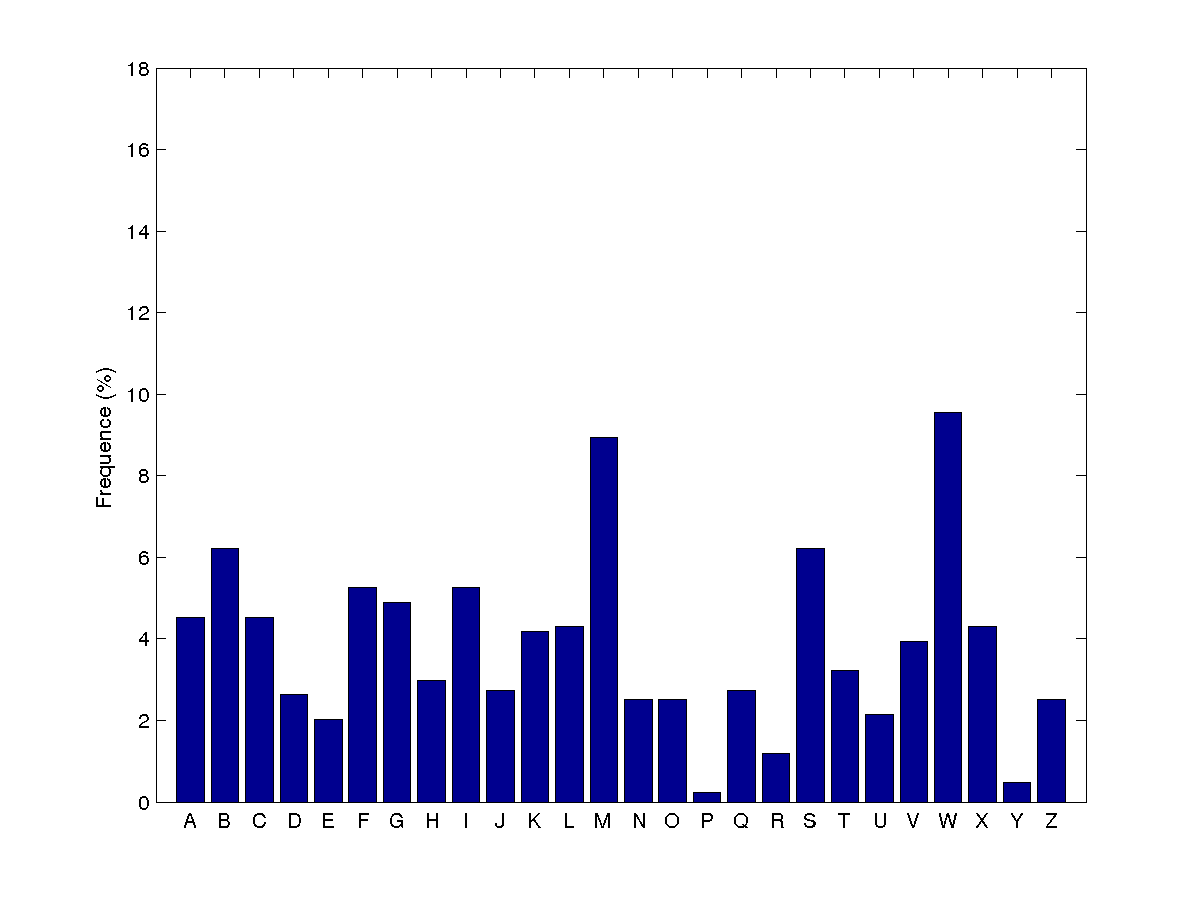
\includegraphics[width=13cm]{img/resVig.png}
\captionof{figure}{Visualisation des fréquences de chaque lettre}
\label{fig3}
\end{minipage} \hfill

\begin{center}
\begin{tabular}{|c|c|c|}
	\hline
	& \textbf{Effectifs} & \textbf{Fréquences}\\
	\hline
	\textbf{Moyenne} &   32.23 &  3.85\\
	\hline
	\textbf{Variance} &  348.90 &  4.97\\
	\hline
	\textbf{Écart-type} &   18.68 &  2.23\\
	\hline
	\textbf{Médiane} &   30.00 &  3.58\\
	\hline
\end{tabular}
\label{tab15}
\captionof{table}{Description des variables}
\end{center}

\begin{center}
\begin{tabular}{|c|}
\hline
\textbf{$IC = 0.0497$}\\
\hline
\end{tabular}
\label{tab16}
\captionof{table}{Indice de coïncidence}
\end{center}

Il est clair que compte tenu de l'histogramme, de la variance et de l'$IC$ aussi différent du français, le chiffre utilisé est poly-alphabétique.
Il sera donc inutile d'étudier les bigrammes de ce texte.

\subsubsection{Pour le cryptogramme n\textdegree3}

\begin{minipage}[c]{.3\linewidth}
  \begin{tabular}{|c|c|c|}
    \hline
	& \textbf{Nb} & \textbf{\%}\\
	\hline
	\textbf{A} &      37 &  7.61\\
	\hline
	\textbf{B} &      48 &  9.88\\
	\hline
	\textbf{C} &       0 &  0.00\\
	\hline
	\textbf{D} &       0 &  0.00\\
	\hline
	\textbf{E} &       6 &  1.23\\
	\hline
	\textbf{F} &      45 &  9.26\\
	\hline
	\textbf{G} &       6 &  1.23\\
	\hline
	\textbf{H} &      30 &  6.17\\
	\hline
	\textbf{I} &       6 &  1.23\\
	\hline
	\textbf{J} &      25 &  5.14\\
	\hline
	\textbf{K} &      16 &  3.29\\
	\hline
	\textbf{L} &       9 &  1.85\\
	\hline
	\textbf{M} &       9 &  1.85\\
	\hline
	\textbf{N} &      21 &  4.32\\
	\hline
	\textbf{O} &      73 &  15.02\\
	\hline
	\textbf{P} &      27 &  5.56\\
	\hline
	\textbf{Q} &      37 &  7.61\\
	\hline
	\textbf{R} &      16 &  3.29\\
	\hline
	\textbf{S} &      37 &  7.61\\
	\hline
	\textbf{T} &      27 &  5.56\\
	\hline
	\textbf{U} &       6 &  1.23\\
	\hline
	\textbf{V} &       1 &  0.21\\
	\hline
	\textbf{W} &       1 &  0.21\\
	\hline
	\textbf{X} &       3 &  0.62\\
	\hline
	\textbf{Y} &       0 &  0.00\\
	\hline
	\textbf{Z} &       0 &  0.00\\
	\hline
	\textbf{Total} &     486 &  100.00\\
	\hline
  \end{tabular}
   \captionof{table}{Résultat des calculs de fréquences}
  \label{tab14}
  \end{minipage}
\begin{minipage}[c]{.85\linewidth}\centering
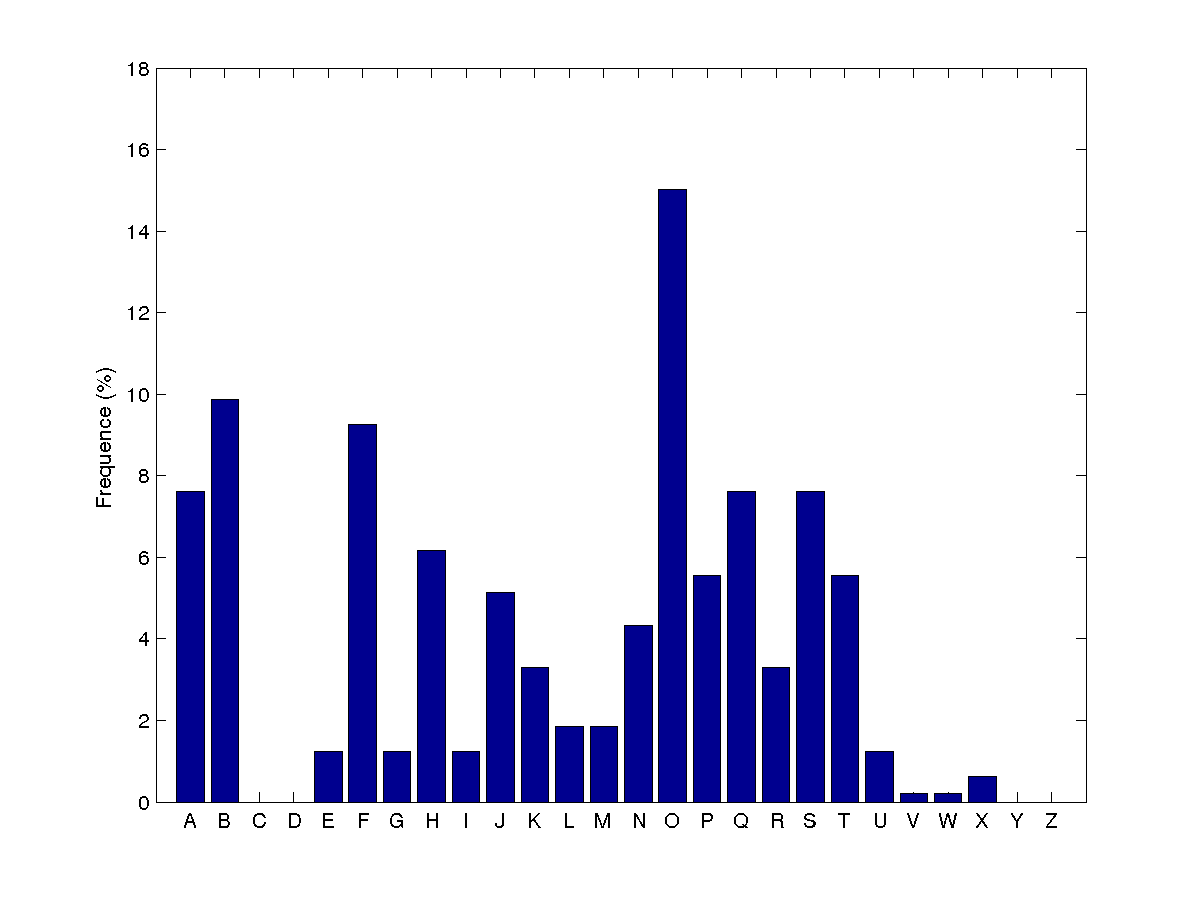
\includegraphics[width=13cm]{img/resMono.png}
\captionof{figure}{Visualisation des fréquences de chaque lettre}
\label{fig4}
\end{minipage} \hfill

\begin{center}
\begin{tabular}{|c|c|c|}
	\hline
	& \textbf{Effectifs} & \textbf{Fréquences}\\
	\hline
	\textbf{Moyenne} &   18.69 &  3.85\\
	\hline
	\textbf{Variance} &  357.34 &  15.13\\
	\hline
	\textbf{Écart-type} &   18.90 &  3.89\\
	\hline
	\textbf{Médiane} &   12.50 &  2.57\\
	\hline
\end{tabular}
\label{tab99}
\captionof{table}{Description des variables}
\end{center}

\begin{center}
\begin{tabular}{|c|}
\hline
\textbf{$IC = 0.0744$}\\
\hline
\end{tabular}
\label{tab56}
\captionof{table}{Indice de coïncidence}
\end{center}

Au vu de ces données, on peut aussi faire l'hypothèse que le cryptosystème utilisé est mono-alphabétique.

\subsection{Fréquence de chaque bigramme dans les cryptogrammes}
Ici encore, on ne s'interessera qu'aux 26 bigrammes les plus fréquents et aux paires de lettres.

\subsubsection{Pour le cryptogramme n\textdegree1}

\begin{center}
\begin{minipage}[c]{.3\linewidth}
\begin{tabular}{|c|c|c|}
 \hline
	& \textbf{Nb} & \textbf{(\%)}\\
	\hline
 	\textbf{CH} &       1 &  4.17\\
	\hline
	\textbf{FG} &       1 &  4.17\\
	\hline
	\textbf{FI} &       1 &  4.17\\
	\hline
	\textbf{FY} &       1 &  4.17\\
	\hline
	\textbf{HN} &       1 &  4.17\\
	\hline
	\textbf{HY} &       1 &  4.17\\
	\hline
	\textbf{IL} &       1 &  4.17\\
	\hline
	\textbf{LM} &       1 &  4.17\\
	\hline
	\textbf{LN} &       1 &  4.17\\
	\hline
	\textbf{LY} &       1 &  4.17\\
	\hline
	\textbf{MI} &       1 &  4.17\\
	\hline
	\textbf{MK} &       1 &  4.17\\
	\hline
	\textbf{NF} &       1 &  4.17\\
	\hline
	\textbf{NU} &       1 &  4.17\\
	\hline
	\textbf{OX} &       1 &  4.17\\
	\hline
	\textbf{OY} &       1 &  4.17\\
	\hline
	\textbf{UF} &       1 &  4.17\\
	\hline
	\textbf{WL} &       1 &  4.17\\
	\hline
	\textbf{YF} &       1 &  4.17\\
	\hline
	\textbf{YH} &       1 &  4.17\\
	\hline
	\textbf{YM} &       1 &  4.17\\
	\hline
	\textbf{YN} &       1 &  4.17\\
	\hline
	\textbf{YP} &       1 &  4.17\\
	\hline
	\textbf{YW} &       1 &  4.17\\
	\hline
	\textbf{AA} &       0 &  0.00\\
	\hline
	\textbf{AB} &       0 &  0.00\\
	\hline
\end{tabular}
   \captionof{table}{Fréquences sur les bigrammes}
  \label{tab98}
\end{minipage}
\begin{minipage}[c]{.3\linewidth}
 \begin{tabular}{|c|c|c|}
 \hline
	& \textbf{Nb} & \textbf{(\%)}\\
	\hline
	\textbf{AA} &       0 &  0.00\\
	\hline
	\textbf{BB} &       0 &  0.00\\
	\hline
	\textbf{CC} &       0 &  0.00\\
	\hline
	\textbf{DD} &       0 &  0.00\\
	\hline
	\textbf{EE} &       0 &  0.00\\
	\hline
	\textbf{FF} &       0 &  0.00\\
	\hline
	\textbf{GG} &       0 &  0.00\\
	\hline
	\textbf{HH} &       0 &  0.00\\
	\hline
	\textbf{II} &       0 &  0.00\\
	\hline
	\textbf{JJ} &       0 &  0.00\\
	\hline
	\textbf{KK} &       0 &  0.00\\
	\hline
	\textbf{LL} &       0 &  0.00\\
	\hline
	\textbf{MM} &       0 &  0.00\\
	\hline
	\textbf{NN} &       0 &  0.00\\
	\hline
	\textbf{OO} &       0 &  0.00\\
	\hline
	\textbf{PP} &       0 &  0.00\\
	\hline
	\textbf{QQ} &       0 &  0.00\\
	\hline
	\textbf{RR} &       0 &  0.00\\
	\hline
	\textbf{SS} &       0 &  0.00\\
	\hline
	\textbf{TT} &       0 &  0.00\\
	\hline
	\textbf{UU} &       0 &  0.00\\
	\hline
	\textbf{VV} &       0 &  0.00\\
	\hline
	\textbf{WW} &       0 &  0.00\\
	\hline
	\textbf{XX} &       0 &  0.00\\
	\hline
	\textbf{YY} &       0 &  0.00\\
	\hline
	\textbf{ZZ} &       0 &  0.00\\
	\hline
\end{tabular}
   \captionof{table}{Fréquences sur les paires}
  \label{tab25}
\end{minipage}
\end{center}

\begin{center}
\begin{tabular}{|c|c|c|}
	\hline
	& \textbf{Effectifs} & \textbf{Fréquences}\\
	\hline
	\textbf{Moyenne} &    0.04 &  0.15\\
	\hline
	\textbf{Variance} &    0.03 &  0.60\\
	\hline
	\textbf{Écart-type} &    0.19 &  0.77\\
	\hline
	\textbf{Médiane} &    0.00 &  0.00\\
	\hline
\end{tabular}
\label{tab32}
\captionof{table}{Description des variables}
\end{center}

Sur un texte aussi petit, on se rend rapidement compte que l'analyse des bigrammes ne sera en rien efficace. 

\subsubsection{Pour le crytogramme n\textdegree3}

\begin{center}
\begin{minipage}[c]{.3\linewidth}
\begin{tabular}{|c|c|c|}
 \hline
	& \textbf{Nb} & \textbf{(\%)}\\
	\hline
	\textbf{AE} &       1 &  0.74\\
	\hline
	\textbf{AF} &       1 &  0.74\\
	\hline
	\textbf{AG} &       1 &  0.74\\
	\hline
	\textbf{AJ} &       1 &  0.74\\
	\hline
	\textbf{AM} &       1 &  0.74\\
	\hline
	\textbf{AN} &       1 &  0.74\\
	\hline
	\textbf{AP} &       1 &  0.74\\
	\hline
	\textbf{AQ} &       1 &  0.74\\
	\hline
	\textbf{AS} &       1 &  0.74\\
	\hline
	\textbf{BA} &       1 &  0.74\\
	\hline
	\textbf{BE} &       1 &  0.74\\
	\hline
	\textbf{BF} &       1 &  0.74\\
	\hline
	\textbf{BH} &       1 &  0.74\\
	\hline
	\textbf{BK} &       1 &  0.74\\
	\hline
	\textbf{BL} &       1 &  0.74\\
	\hline
	\textbf{BP} &       1 &  0.74\\
	\hline
	\textbf{BR} &       1 &  0.74\\
	\hline
	\textbf{BS} &       1 &  0.74\\
	\hline
	\textbf{BT} &       1 &  0.74\\
	\hline
	\textbf{BW} &       1 &  0.74\\
	\hline
	\textbf{EF} &       1 &  0.74\\
	\hline
	\textbf{EJ} &       1 &  0.74\\
	\hline
	\textbf{EO} &       1 &  0.74\\
	\hline
	\textbf{EP} &       1 &  0.74\\
	\hline
	\textbf{FB} &       1 &  0.74\\
	\hline
	\textbf{FF} &       1 &  0.74\\
	\hline
\end{tabular}
   \captionof{table}{Fréquences sur les bigrammes}
  \label{tab34}
\end{minipage}
\begin{minipage}[c]{.3\linewidth}
 \begin{tabular}{|c|c|c|}
 \hline
	& \textbf{Nb} & \textbf{(\%)}\\
	\hline
	\textbf{AA} &       0 &  0.00\\
	\hline
	\textbf{BB} &       0 &  0.00\\
	\hline
	\textbf{CC} &       0 &  0.00\\
	\hline
	\textbf{DD} &       0 &  0.00\\
	\hline
	\textbf{EE} &       0 &  0.00\\
	\hline
	\textbf{FF} &       1 &  0.74\\
	\hline
	\textbf{GG} &       0 &  0.00\\
	\hline
	\textbf{HH} &       1 &  0.74\\
	\hline
	\textbf{II} &       0 &  0.00\\
	\hline
	\textbf{JJ} &       0 &  0.00\\
	\hline
	\textbf{KK} &       1 &  0.74\\
	\hline
	\textbf{LL} &       0 &  0.00\\
	\hline
	\textbf{MM} &       0 &  0.00\\
	\hline
	\textbf{NN} &       0 &  0.00\\
	\hline
	\textbf{OO} &       0 &  0.00\\
	\hline
	\textbf{PP} &       0 &  0.00\\
	\hline
	\textbf{QQ} &       0 &  0.00\\
	\hline
	\textbf{RR} &       0 &  0.00\\
	\hline
	\textbf{SS} &       0 &  0.00\\
	\hline
	\textbf{TT} &       0 &  0.00\\
	\hline
	\textbf{UU} &       1 &  0.74\\
	\hline
	\textbf{VV} &       0 &  0.00\\
	\hline
	\textbf{WW} &       0 &  0.00\\
	\hline
	\textbf{XX} &       0 &  0.00\\
	\hline
	\textbf{YY} &       0 &  0.00\\
	\hline
	\textbf{ZZ} &       0 &  0.00\\
	\hline
\end{tabular}
   \captionof{table}{Fréquences sur les paires}
  \label{tab29}
\end{minipage}
\end{center}

\begin{center}
\begin{tabular}{|c|c|c|}
	\hline
	& \textbf{Effectifs} & \textbf{Fréquences}\\
	\hline
	\textbf{Moyenne} &    0.20 &  0.15\\
	\hline
	\textbf{Variance} &    0.16 &  0.09\\
	\hline
	\textbf{Écart-type} &    0.40 &  0.30\\
	\hline
	\textbf{Médiane} &    0.00 &  0.00\\
	\hline
\end{tabular}
\label{tab187}
\captionof{table}{Description des variables}
\end{center}

Là encore, l'analyse ne nous sera pas très utile (l'effectif des bigrammes les plus fréquents est toujours de $1$).
Mais, l'étude des paires de lettres pourra nous aider.

\newpage
\subsection{Les mots les plus fréquents du français}

Après un script de récupération des effectifs de chaque mot et un petit traitement MatLab\footnote{En annexe} pour déterminer les $20$ mots (de plus de deux lettres) les plus fréquents dans le texte, on a le résultat suivant :\\

\begin{center}
\begin{tabular}{|c|c|c|}
 \hline
	& \textbf{Nb} & \textbf{(\%)}\\
	\hline
		\textbf{LES} &   12940 &  1.81\\
	\hline
	\textbf{QUE} &    8184 &  1.14\\
	\hline
	\textbf{CES} &    7905 &  1.11\\
	\hline
	\textbf{QUI} &    6679 &  0.93\\
	\hline
	\textbf{UNE} &    5893 &  0.82\\
	\hline
	\textbf{DANS} &    5428 &  0.76\\
	\hline
	\textbf{ÉTAIT} &    4528 &  0.63\\
	\hline
	\textbf{PAS} &    4495 &  0.63\\
	\hline
	\textbf{ELLE} &    4202 &  0.59\\
	\hline
	\textbf{SON} &    3840 &  0.54\\
	\hline
	\textbf{POUR} &    3720 &  0.52\\
	\hline
	\textbf{SUR} &    3682 &  0.51\\
	\hline
	\textbf{PLUS} &    3477 &  0.49\\
	\hline
	\textbf{PAR} &    3474 &  0.49\\
	\hline
	\textbf{LUI} &    3156 &  0.44\\
	\hline
	\textbf{MAIS} &    2839 &  0.40\\
	\hline
	\textbf{COMME} &    2786 &  0.39\\
	\hline
	\textbf{AVAIT} &    2712 &  0.38\\
	\hline
	\textbf{TOUT} &    2608 &  0.36\\
	\hline
	\textbf{VOUS} &    2592 &  0.36\\
	\hline
\end{tabular}
   \captionof{table}{Fréquences sur les mots}
  \label{tab74}
\end{center}

\chapter{Application aux codes secrets}
Dans cette partie, on essaiera de déchiffrer les textes codés.
On utilisera principalement des techniques qui s'appliquent à un chiffre de substitution mono-alphabétique, car pour déchiffrer le code de Vigenère on se ramène à ce cas particulier.
Pour cela, nous devrons faire des hypothèses sur ces textes grâce aux données précédemment présentées, par exemple :
\begin{center}
 $\mathcal{H} $ : \og Dans ce cryptogramme, la lettre \emph{E} représente la lettre \emph{y} \fg{}.
\end{center}
Nous aurons donc besoin d'outils qui évaluent la véracité de telles suppositions.
Nous pourrons enfin appliquer ces hypothèses aux chiffres.

\section{Test des hypothèses en cryptanalyse}

Dans cette partie, on appelera :
\begin{itemize}
	\item E un ensemble d'éléments (par exemple les monogrammes, les bigrames, …, les mots)
	\item Objet $o \in E$ un élément de $E$ (par exemple, un monogramme, un bigramme, etc.)
	\item $O$ la variable aléatoire qui représente un objet (par exemple, si on est dans l'ensemble des monogrammes $\mathbb{P}(O = a)$ est la probabilité de tomber sur le monogramme $a$)
\end{itemize}

On va donc appliquer des tests qui compareront $\mathbb{P}(O = o)$, que l'on a estimé, et la fréquence d'apparition de chaque objets dans un cryptogramme.,

\subsection{Distance entre deux éléments}
\subsubsection{L'hypothèse à vérifier}
On cherche à évaluer si un élément (monogramme, bigramme, etc.) du texte chiffré est en relation avec un élément de la langue française.
Autrement dit, on s'intéresse aux hypothèses suivantes :
\begin{itemize}
 \item $\mathcal{H}_{0}$ : \og L'objet $o$ de la langue française est chiffré par l'objet $o'$ dans le cryptogramme \fg{}
 \item $\mathcal{H}_{1}$  : \og L'objet $o$ de la langue française n'est pas chiffré par l'objet $o'$ dans le cryptogramme \fg{}
\end{itemize}

\subsubsection{Définition}
L'approche la plus intuitive est d'évaluer l'écart de la fréquence d'apparition de chacun de ces éléments :
\[d(o, o') = |\hat{P}(O = o)_{cryptogramme} - \mathbb{P}(O = o')|\]

Pour avoir un nombre plus significatif, on préférera prendre l'écart entre les effectifs. 
Dans un texte de $n$ objets, on compte $n_{o}$ le nombre d'apparitions de l'objet $o$. 
On connaît $\mathbb{P}(O = o')$ que l'on a évalué dans la première partie.
Et donc, 
\[d(o, o') = |n_{o} - n\times \mathbb{P}(O = o')|\]

Pour trouver l'objet $o'$ qui est le plus probablement représentatif de l'objet $o$, il suffit de trouver celui qui minimise $d(o,o')$.

\subsection{Forme d'un texte}
\subsubsection{L'hypothèse à vérifier}
La forme va nous servir à évaluer ce genre d'hypothèses :
\begin{itemize}
 \item $\mathcal{H}_{0}$ : \og Le cryptogramme est déchiffré \fg{}
 \item $\mathcal{H}_{1}$  : \og Le cryptogramme n'est pas déchiffré \fg{}
\end{itemize}

\subsubsection{Définition}
La forme d'un texte évalue concrètement la différence qu'il existe entre ce texte par rapport à un texte source.
Typiquement, si l'on déchiffre un texte de plusieurs façons différentes, cet outil nous indiquera quel est le déchiffrement le plus proche de la langue.
Dans notre cas, donc, on utilisera cet outil statistique en prenant pour texte source celui étudié précédemment qui dépeint correctement la langue française.

La forme est définie d'après la probabilité d'apparition des n-grammes ou des mots du texte source.
En pratique :
\begin{itemize}
 \item On choisit l'ensemble d'objets $E$ à étudier : monogrammes, bigrammes, trigrammes, … mots.
 \item On calcule la fréquence d'apparition de chaque objet $O_{i}$ dans le texte source, on considère alors que cette fréquence est une très bonne estimation de $\mathbb{P}(O = O_{i})$.
\end{itemize}

La forme du texte étudié est ensuite définie par la formule suivante :
\[ \gamma = \prod \limits_{\substack{{O_{i} \in texte} \\ O_{i} \neq O_{j}}} \mathbb{P}(O = O_{i})^{n_{i}} \]
Avec $n_{i}$ le nombre d'apparition de $O_{i}$ dans le texte dont on calcule la forme et $\mathbb{P}(O = O_{i})$ la probabilité d'apparition de $O_{i}$ dans le texte source.
Autrement dit, c'est le produit des probabilités d'apparition dans le texte source de chaque objet du texte étudié.
Pour des raisons pratiques, on préfère prendre le logarithme de la forme :
\[ \Gamma = log(\gamma) = log(\prod \limits_{\substack{{O_{i} \in texte} \\ O_{i} \neq O_{j}}}  \mathbb{P}(O = O_{i})^{n_{i}}) = \sum \limits_{\substack{{O_{i} \in texte} \\ O_{i} \neq O_{j}}}  n_{i} \times log(\mathbb{P}(O = O_{i}))\]
En effet, le nombre produit étant compris entre $0$ et $1$, un logarithme nous permet de mieux l'évaluer.

\subsubsection{Analyse de la forme}

On a un outil, c'est bien. Encore faut-il savoir ce qu'il signifie.
On se base par exemple sur la probabilité d'apparition de chaque bigramme en français.
Supposons que l'on ait deux textes de même longueur : l'un ne signifie absolument rien (exemple : \og ABNNK SETAS CPOAE ANBME EBINS JCLVY X \fg{}) et l'autre veut dire quelque chose de terriblement profond (exemple : \og Est-ce que votre blanquette est bonne ? \fg{}).
La forme non-logarithmique $\gamma$ du premier texte sera très proche de $0$ car les bigrammes qui le composent n'apparaissent presque pas en français.
Alors que, pour l'autre texte, $\gamma$ sera moins proche de $0$ que le premier.

Lorsque l'on applique le logarithme, donc, la forme du premier texte $\Gamma$ sera très négative, alors que pour le second texte elle sera plus élevée (mais toujours négative).

Finalement :
\begin{center}
 \emph{Plus $\Gamma$ est grand, plus le texte est susceptible d'être en français.}
\end{center}

Casser le chiffre, c'est donc essayer de maximiser $\Gamma$.
Une dernière remarque : évidemment, selon les objets que l'on étudie (monogrammes, bigrammes, etc.), la précision de la forme sera plus ou moins intéressante.
Avec des quadrigrammes ou des mots, la forme sera très précise, alors qu'avec des monogrammes elle est un peu moins révélatrice.
On se contentera des monogrammes puis des bigrammes : c'est déjà assez précis, et on ne peut pas se permettre de travailler avec des mots car le cryptographe ne nous a pas rendu la tâche facile : il a séparé son cryptogramme en bloc de $5$ lettres de façon à ce que l'on ne puisse pas discerner les mots.

\subsection{Ce bon vieux $\chi^{2}$}
\subsubsection{L'hypothèse à vérifier}
Le test du $\chi^{2}$ va nous servir aussi à évaluer ces hypothèses :
\begin{itemize}
 \item $\mathcal{H}_{0}$ : \og Le cryptogramme est déchiffré \fg{}
 \item $\mathcal{H}_{1}$  : \og Le cryptogramme n'est pas déchiffré \fg{}
\end{itemize}

\subsubsection{Le test d'adéquation}
En statistiques, le test de $\chi^{2}$ sert à évaluer s'il y a une relation entre des variables qualitatives.
Autrement dit, il sert à tester l'indépendance de ces variables.
Dans notre cas, on va l'utiliser pour tester l'adéquation entre l'apparition de certains objets dans un cryptogramme (monogrammes, bigrammes, etc.) avec leur apparition théorique (c'est-à-dire en français).

On notera $E$ l'ensemble des objets étudiés, $n_{i}$ le nombre d'apparitions de l'objet $O_{i}$ dans le cryptogramme composé de $n$ objets.

On définit alors la statistique du $\chi^{2}$ : 
\[D(Observations, Theorie) = \sum \limits_{\substack{{O_{i} \in texte} \\ O_{i} \neq O_{j}}}  \frac{(n_{i} - n \times \mathbb{P}(O = O_{i}))^{2}}{n \times \mathbb{P}(O = O_{i})} = \sum \limits_{\substack{{O_{i} \in texte} \\ O_{i} \neq O_{j}}}  \frac{d(O_{i},O_{i})^{2}}{n \times \mathbb{P}(O = O_{i})} \]

Sous l'hypothèse $\mathcal{H}_{0}$ : \og Le cryptogramme est déchiffré \fg{}, c'est-à-dire si toutes les probabilités d'apparition des $O_{i}$ du cryptogramme sont égales aux probabilités d'apparition des $O_{i}$ théoriques, cette statistique suit une loi du $\chi^{2}$ à $card(E) - 1$ degrés de liberté.
On pourra donc se ramener aux tables du $\chi^{2}$ pour récupérer la p-valeur.

On utilisera cette formule ici uniquement pour les monogrammes, ce qui revient à écrire : 
\[D(Observations, Theorie) = \sum_{l = A}^{Z}  \frac{(n_{l} - n \times \mathbb{P}(L = l))^{2}}{n \times \mathbb{P}(L = l)} = \sum_{l = A}^{Z}  \frac{d(l,l)^{2}}{n \times \mathbb{P}(L = l)}\]
Et donc, sous l'hypothèse $\mathcal{H}_{0}$, la loi du $\chi^{2}$ suivie est à $25$ degrès de liberté.

\subsection{Analyse de tout cela}

Résoudre notre problème, c'est-à-dire casser le chiffre, c'est donc minimiser $D$ (ce qui revient à minimiser chaque écart $d$) \textbf{et} maximiser $\Gamma$.
Le test de la forme va évaluer si le texte déchiffré est du charabia ou non, alors que le $\chi^{2}$ nous dira si l'on est en adéquation avec les probabilités théoriques d'apparition.

La solution aura donc une forme élevée (si ce n'est la plus élevée), mais pas forcément le plus petit $D$ possible.
En effet, G. Perec a bien écrit un livre sans utiliser une seule fois la lettre $e$ : \emph{La disparition}, qui est pourtant la lettre la plus utilisée en français. La distance du $\chi^{2}$ nous induirait en erreur dans ce cas.


\section{Les cryptogrammes mono-alphabétiques}
Pour chacun de ces cryptogrammes, nous procéderons de la manière suivante : 
\begin{itemize}
\item On tentera une attaque par force brute en essayant les 25 clés possibles dans le cas d'un chiffrement César.
\item Si cela ne fonctionne pas, on utilisera un algorithme utilisant la forme pour casser le chiffre mono-alphabétique automatiquement.
\item Là encore, si le cryptogramme est toujours incompréhensible, on gardera le traitement précédent (qui sera presque correct en théorie), et on se débrouillera à la main en essayant de minimiser la distance du $\chi^{2}$.
\end{itemize}

\subsection{Cryptogramme n\textdegree1}

Pour rappel, on veut savoir ce qu'il se trame derrière cette expression :
\begin{center}
\begin{quote}
\og FILMK OYFYP CHYHN LYFYM YWLYN MILNF YNUFG OX \fg{}
\end{quote}
\end{center}

\subsubsection{Tentative d'attaque par force brute}

On applique un programme Pascal\footnote{Disponible en annexe} au cryptogramme pour en déduire tous les textes \og décalés \fg{} de César.
Après calcul des formes du texte et de la distance du $\chi^{2}$, on a :
\begin{center}
\begin{tabular}{|c|c|c|c|c|c|}
 \hline
	\textbf{clé}& \textbf{texte} & \textbf{Forme (mono)} & \textbf{Forme (big)} & \textbf{$D$} & \textbf{p-valeur (\%)}\\
	\hline
	\textbf{1} & ehkljnxexobg... &  -167 & -460 & 3455 & $\simeq$ 0\\
	\hline
	\textbf{2} & dgjkimwdwnaf... &  -193 & -477 & 17867 & $\simeq$ 0\\
	\hline
	\multicolumn{6}{|c|}{\textbf{...}}\\
	\hline
	\textbf{20} & lorsquelevi... &   -98 & -189 & 13 & 98 \\
	\hline
	\multicolumn{6}{|c|}{\textbf{...}}\\
	\hline
	\textbf{25} & gjmnlpzgzqd... &  -161 & -440 & 1109 & $\simeq$ 0\\
	\hline
\end{tabular}
   \captionof{table}{Test de toutes les clés du chiffre de César}
  \label{tab77}
\end{center}
Eurêka ! Ça fonctionne : le texte déchiffré est sûrement le $20^{eme}$, car la forme est plus élevée mais aussi parce que la distance du $\chi^{2}$ est faible. En effet on a une p-valeur élevée, ici on a environ $98\%$ de chances d'avoir un texte plus distant du français que celui-là, ce qui est très correct.
Finalement, la $20^{eme}$ clé révèle bien le secret suivant : 

\begin{center}
\begin{quote}
\og Lorsque le vin entre, le secret sort - Le Talmud\fg{}
\end{quote}
\end{center}

One down, two to go.

\subsection{Cryptogramme n\textdegree3}

On rappelle que l'on cherche à cryptanalyser ce texte :
\begin{center}
\begin{quote}
\og OHQSB SAQSA MTOQF BFJAN OQLPB HNQHJ GEPOQ OHBHL FBAQF BWJUF BPLOH TGEOP QBEPL FFHOX KPAGO FOUBA SMTOF OQRBP BRSPA QSAMT OQNTH RIBHS AFFJH BFBSJ APOQO PBKKP JRIOH SNBTS BHSKF TQNOQ RBPBR SPAQS AMTOQ QSBSA QSAMT OQNOF BKJKT FBSAJ HMTOF BSBAF FONOF RIBHS AFFJH BTLGO HSOFB SBAFF ONOFR IBHSA FFJHR JHQAN POPKJ TPBKK PJRIO PFOQR BPBRS PAQSA MTOQN OFBKJ KTFBS AJHHO NKOHN MTOUB AEFOG OHSVJ APOKB QNTSJ TSNOF BSBAF FONOR OFFOR AMTOF OQJHN BLOQJ ASUBA SBTFT XOGEJ TPLJT BTXSB SQTHA QAFQT UUASK JTPJE SOHAP NOQKP RAQAJ HQLBF OQNOK POHNP ONOQR IBHSA FFJHQ NOSBA FFOQL BFOQ \fg{}
\end{quote}
\end{center}

\subsubsection{Tentative d'attaque par force brute}
Les résultats de l'attaque sur le cryptogramme sont les suivants :
\begin{center}
\begin{tabular}{|c|c|c|c|c|c|}
 \hline
	\textbf{clé}& \textbf{texte} & \textbf{Forme (mono)} & \textbf{Forme (big)} & \textbf{$D$} & \textbf{p-valeur (\%)}\\
	\hline
	\textbf{1} & ngprarzprzls... &   -1628 & -4396 & 3321 & $\simeq$ 0\\
	\hline
	\textbf{2} & mfoqzqyoqykr... &  -1907 & -5470 & 5307 & $\simeq$ 0\\
	\hline
	\multicolumn{6}{|c|}{\textbf{...}}\\
	\hline
	\textbf{25} & pirtctbrtbn... &  -1780 & -4855 & 9546 & $\simeq$ 0\\
	\hline
\end{tabular}
   \captionof{table}{Test de toutes les clés du chiffre de César}
  \label{tab78}
\end{center}
Sacrebleu ! Cela ne donne rien !
Sortons l'artillerie lourde.

\subsubsection{Utilisation d'un algorithme Hill-Climbing}

Bon, vu d'ici, on pourrait procéder de $3$ manières différentes :
\begin{itemize}
\item Essayer de casser le chiffre à la main en utilisant les fréquences précédemment calculées : en \og tâtonnant \fg{}.
\item Tenter une attaque par force brute sur les $26!$ clés possibles avec un ordinateur.
\item Tenter une attaque, via l'outil informatique aussi, mais de façon à minimiser le nombre d'itérations.
\end{itemize}

Les deux dernières solutions sont intéressantes car elles automatisent le déchiffrement.
Toutefois, la deuxième solution est gourmande en ressources : elle demande d'effectuer de l'ordre de $26!$ itérations. Et, les ressources, en cryptanalyse c'est important : pour casser RSA\footnote{Un cryptosystème récent et très utilisé du fait de sa praticité et de sa sécurité} avec une machine puissante, il faut compter plusieurs années pour une clé de 768 bits (et on utilise aujourd'hui surtout des clés de 2048 bits…).
Nous allons donc opter pour la troisième solution.

Nous utiliserons un algorithme de type \emph{Hill-Climbing}\footnote{C'est un algorithme qui modifie une solution fausse jusqu'à en trouver une bonne} en utilisant la forme du texte.
Son fonctionnement sera le suivant :
\begin{enumerate}
\item Générer une clé aléatoire (qui, ici, est un alphabet) et la tester en calculant la forme du texte ainsi déchiffré.
\item Échanger au hasard deux caractères de la clé, la tester de la même manière. 
\item Si la nouvelle forme est plus grande que la précédente, on change la clé par la clé permutée.
\item On retourne à l'étape 2, sauf si l'on a fait 1000 itérations sans changer de clé.
\end{enumerate}

On relance cet algorithme jusqu'à obtenir une forme qui soit sensiblement proche d'un texte français comportant le même nombre de caractères.
Autrement dit, nous avons besoin de calculer une forme \og correcte \fg{} vers laquelle on veut que l'algorithme tende.
Calculer cette forme \og basique \fg{} est relativement simple.
Rappelons la formule de la forme :
\[ \Gamma = \sum \limits_{\substack{{O_{i} \in texte} \\ O_{i} \neq O_{j}}}  n_{i} \times log(\mathbb{P}(O = O_{i}))\]
Avec $n_{i}$ le nombre d'apparitions de l'objet $O_{i}$ dans le texte étudié.
Pour avoir une forme correcte, il faut que chaque fréquence des objets du texte suive la même loi de probabilité que ces objets en français.
Autrement dit, en notant $n$ le nombre d'objets dans le texte, la forme recherchée est la suivante :
\[ \Gamma_{0} = \sum \limits_{\substack{{O_{i} \in texte} \\ O_{i} \neq O_{j}}}  n \times \mathbb{P}(O = O_{i}) \times log(\mathbb{P}(O = O_{i}))\]

La condititon d'arrêt sera donc la suivante : forme $\geq$ forme basique.

On implémente cet algorithme en Pascal\footnote{Disponible en annexe}, avec la forme des bigrammes (qui est plus précise) et on obtient la clé suivante (au bout d'une petite vingtaine de minute de recherche itérative) : 

\begin{center}
  \begin{tabular}{p{1.5cm}*{26}{p{0.1cm}}}
    \hline
    \textbf{Alphabet clair} & a & b & c & d & e & f & g & h & i & j & k & l & m & n & o & p & q & r & s & t & u & v & w & x & y & z \\
    \hline
    \textbf{Alphabet chiffré} & B & I & N & G & O & U & E & V & A & W & Z & F & R & H & J & K & M & P & Q & S & T & L & D & X & Y & C \\
    \hline
  \end{tabular}
   \captionof{table}{Clé trouvée par l'algorithme Hill-Climbing}
  \label{tab432} 
\end{center}

Ce qui donne ce texte déchiffré :

\begin{center}
\begin{quote}
\og ENSTATISTIQUESLALOICESVRANCSNODGRESENANVLAISLAJOFLARVENUDGERS
AGREVELLNEXPRIDELEFAITQUELESMARAMTERISTIQUESCUNEMBANTILLONALEATOIRE
SERAPPROMBENTCAUTANTPLUSCESMARAMTERISTIQUESSTATISTIQUESCELAPOPULATION
QUELATAILLECELEMBANTILLONAUVDENTELATAILLECELEMBANTILLONAMONSICERERPOUR
APPROMBERLESMARAMTERISTIQUESCELAPOPULATIONNECEPENCQUEFAIGLEDENTHOIREPAS
CUTOUTCELATAILLECEMELLEMIQUELESONCAVESOITFAITAULUXEDGOURVOUAUXETATSUNIS
ILSUFFITPOUROGTENIRCESPREMISIONSEVALESCEPRENCRECESEMBANTILLONSCETAILLESEVALES \fg{}
\end{quote}
\end{center}

Ça marche bien !
On reconnaît du français un peu partout dans le texte.
On réécrit ce même texte en mettant en minuscules les caractères que l'on suppose correctement déchiffrés :

\begin{center}
\begin{quote}
\og en statistiques la loi CesVranCsnoDGresenanVlaislaJoflarVenuDGersaGreVellneXpriDe le fait que les MaraMteristiquesCuneMBantillon aleatoire serapproMBentC autant plus CesMaraMteristiques statistiques Cela population que la taille CeleMBantillonauVDente la taille CeleMBantillonaMonsiCerer pour approMBerlesMaraMteristiquesCela population neCepenCquefaiGleDentHoirepasCutoutCe la taille CeMelleMiquelesonCaVe soit fait au luXeDGourVouauX etats unis il suffit pour oGtenirCespreMisionseValesCeprenCreCeseMBantillonsCe tailles eVales \fg{}
\end{quote}
\end{center}

Ce qui \og fixe \fg{} dans la clé les caractères suivants :

\begin{center}
  \begin{tabular}{p{1.5cm}*{26}{p{0.1cm}}}
    \hline
    \textbf{Alphabet clair} & a & b & c & d & e & f & g & h & i & j & k & l & m & n & o & p & q & r & s & t & u & v & w & x & y & z \\
    \hline
    \textbf{Alphabet chiffré} & \textbf{B} & I & N & G & \textbf{O} & \textbf{U} & E & V & \textbf{A} & W & Z & \textbf{F} & R & \textbf{H} & \textbf{J} & \textbf{K} & \textbf{M} & \textbf{P} & \textbf{Q} & \textbf{S} & \textbf{T} & L & D & X & Y & C \\
    \hline
  \end{tabular}
   \captionof{table}{Même clé avec les caractères de la clé supposés corrects en gras}
  \label{tab431} 
\end{center}

\subsubsection{Déchiffrement du reste du cryptogramme}

Nous avons \og quasiment \fg{} déchiffré le texte en maximisant la forme, nous allons maintenant essayer de minimiser la distance du $\chi^{2}$.
Voici le tableau des fréquences de chaque lettre dans le cryptogramme en partie déchiffré, ainsi que leurs fréquences estimées en français (en pourcents). Les lettres en gras sont supposées correctement déchiffrées (ce sont les lettres au-dessus des caractères considérés corrects de la clé) :

\begin{center}
\begin{tabular}{|c|c|c|c|}
\hline
\textbf{Lettre} & \textbf{Français} & \textbf{Cryptogramme} & \textbf{Distance d}\\
\hline
  \textbf{A} & 8.59 &  9.87  &  6.24\\
\hline
  $B$ & 1.01 &     1.23 &  1.06\\
\hline
  $C$ & 3.07 &     4.32 &  6.05\\
\hline
  $D$ & 3.70 &     1.23 &  1.99\\
\hline
    \textbf{E}  & 17.17 &    15.0 &  0.14 \\
\hline
    \textbf{F}  & 1.10 &     1.23 &  0.63\\
\hline
  $G$ & 1.07 &     1.23 &  0.78\\
\hline
  $H$ & 1.00 &     0.20 &  3.86\\
\hline
    \textbf{I}  & 7.35 &     7.61 &  1.23\\
\hline
  $J$ & 0.41 &     0.20 &  1.03\\
\hline
  $K$ & 0.01 &     0.00 &  0.07\\
\hline
    \textbf{L}  & 5.91 &     9.25 &  6.23\\
\hline
  $M$ & 2.78 &     3.29 &  2.44\\
\hline
    \textbf{N}  & 6.91 &     6.17 &  3.60\\
\hline
  \textbf{O} & 5.32 &     5.14 &  0.89\\
\hline
  \textbf{P} & 2.70 &     3.29 &  2.86\\
\hline
    \textbf{Q}  & 1.17 &     1.85 &  3.27\\
\hline
    \textbf{R}  & 6.56 &     5.55 &  4.90\\
\hline
    \textbf{S}  & 7.89 &     7.61 &  1.39\\
\hline
    \textbf{T}  & 7.31 &     7.61 &  1.44\\
\hline
    \textbf{U}  & 6.35 &     5.55 &  3.90\\
\hline
   $V$ & 1.59 &     1.85 &  1.24\\
\hline
   $W$ & 0.01 &     0.00 &  0.05\\
\hline
   $X$ & 0.42 &     0.61 &  0.93\\
\hline
   $Y$ & 0.35 &     0.00 &  1.73\\
\hline
   $Z$ & 0.17 &     0.00 &  0.83\\
\hline
  \end{tabular}
   \captionof{table}{Comparaison des fréquences d'apparition de chaque lettre}
  \label{tab232}
\end{center}

\begin{center}
\begin{tabular}{|c|}
\hline
\textbf{$D = 33.82$}\\
\hline
\end{tabular}
\label{tab10}
\captionof{table}{Distance du $\chi^{2}$}
\end{center}

On a donc une p-valeur de 11\%.
On voit dans ce tableau que, parmi les lettres considérées comme n'étant pas encore déchiffrées, la fréquence du $C$ n'est pas très proche de celle du français.
Revenons sur le texte en partie déchiffré :

\begin{center}
\begin{quote}
\og en statistiques la loi \textbf{Ces} VranCsnoDGresenanVlaislaJoflarVenuDGersaGreVellneXpriDe le fait que les MaraMteristiquesCuneMBantillon aleatoire serapproMBent \textbf{C autant} plus \textbf{Ces} MaraMteristiques statistiques \textbf{Ce} la population que la taille CeleMBantillonauVDente la taille CeleMBantillonaMonsiCerer pour approMBerlesMaraMteristiques \textbf{Ce} la population neCepenCquefaiGleDentHoirepas \textbf{Cu} tout \textbf{Ce} la taille CeMelleMiquelesonCaVe soit fait au luXeDGourVouauX etats unis il suffit pour oGtenirCespreMisionseValesCeprenCreCeseMBantillonsCe tailles eVales \fg{}
\end{quote}
\end{center}

On voit ici que le $C$ pourrait très bien représenter la lettre $d$ en français.
Calculons la distance entre $C$ et $d$ pour tester cette hypothèse :
\[ d(C,d) = |21 - 486\times0,0370| = 3,018 \]
Ce n'est pas top, mais c'est toujours mieux que la distance $d(C,c)$, on va donc supposer cette hypothèse comme étant juste.

Le cryptogramme devient alors :

\begin{center}
\begin{quote}
\og en statistiques la loi des VrandsnoDGresenanVlaislaJoflarVenuDGersaGreVellneXpriDe le fait que les MaraMteristiques dune MBantillon aleatoire serapproMBent d autant plus des MaraMteristiques statistiques de la population que la taille de leMBantillonauVDente la taille de leMBantillonaMonsiderer pour approMBerlesMaraMteristiques de la population ne depend que faiGleDentHoire pas du tout de la taille de MelleMiquelesondaVe soit fait au luXeDGourVouau etats unis il suffit pour oGtenir des preMisionseVales de prendre des eMBantillons de tailles eVales \fg{}
\end{quote}
\end{center}

Cela semble correct aussi.

On échange dans la clé le caractère en-dessous du $c$ par celui qui est en-dessous du $d$. (Ce qui, auparavant, était traduit par un $c$ dans le cryptogramme, est maintenant traduit par un $d$).
La clé devient donc :

\begin{center}
  \begin{tabular}{p{1.5cm}*{26}{p{0.1cm}}}
    \hline
    \textbf{Alphabet clair} & a & b & c & d & e & f & g & h & i & j & k & l & m & n & o & p & q & r & s & t & u & v & w & x & y & z \\
    \hline
    \textbf{Alphabet chiffré} & \textbf{B} & I & G & \textbf{N} & \textbf{O} & \textbf{U} & E & V & \textbf{A} & W & Z & \textbf{F} & R & \textbf{H} & \textbf{J} & \textbf{K} & \textbf{M} & \textbf{P} & \textbf{Q} & \textbf{S} & \textbf{T} & L & D & X & Y & C \\
    \hline
  \end{tabular}
   \captionof{table}{Nouvelle clé}
  \label{tab4316} 
\end{center}


\begin{center}
\begin{tabular}{|c|}
\hline
\textbf{$D = 29.28$}\\
\hline
\end{tabular}
\label{tab10}
\captionof{table}{Nouvelle distance du $\chi^{2}$}
\end{center}
Cela donne une p-valeur de 25\%, ce qui est finalement bien plus correct.
Impossible de deviner le mot-clé pour l'instant.
On peut même être amené à se demander \og Y a-t-il un mot-clé ? Ou est-ce juste un alphabet ? \fg{}
En fait, il est très probable que le texte soit chiffré avec un mot clé. 
Si l'on regarde les lettres fixées dans la clé on peut voir une suite de lettre : \og \textbf{F}R\textbf{HJKMPQST} \fg{} qui semble presque correspondre à un morceau de l'alphabet dont on a enlevé quelques lettres : comme lors d'un chiffrement par mot-clé !
En suivant cette intuition, on peut en déduire que la lettre à côté du $F$ fixé se doit d'être un $G$.
Cela donne, en échangeant le $R$ à côté du $F$ par le $G$ en-dessous du $c$ :

\begin{center}
  \begin{tabular}{p{1.5cm}*{26}{p{0.1cm}}}
    \hline
    \textbf{Alphabet clair} & a & b & c & d & e & f & g & h & i & j & k & l & m & n & o & p & q & r & s & t & u & v & w & x & y & z \\
    \hline
    \textbf{Alphabet chiffré} & \textbf{B} & I & R & \textbf{N} & \textbf{O} & \textbf{U} & E & V & \textbf{A} & W & Z & \textbf{F} & \textbf{G} & \textbf{H} & \textbf{J} & \textbf{K} & \textbf{M} & \textbf{P} & \textbf{Q} & \textbf{S} & \textbf{T} & L & D & X & Y & C \\
    \hline
  \end{tabular}
   \captionof{table}{Nouvelle clé}
  \label{tab4131} 
\end{center}

Ce qui donne au niveau du cryptogramme :

\begin{center}
\begin{quote}
\og en statistiques la loi des VrandsnomGresenanVlaislaJoflarVenumGersaGreVelln \textbf{eXprime} le fait que les CaraCteristiques dune CBantillon aleatoire serapproCBent d autant plus des \emph{CaraCteristiques} statistiques de la population que la taille de leCBantillonauVmente la taille de leCBantillonaConsiderer pour approCBerlesCaraCteristiques de la population ne depend que faiGlementHoire pas du tout de la taille deCelleCiquelesondaVe soit fait au luXemGourVouau etats unis il suffit pour oGtenir des \textbf{preCisions} eVales de prendre des eCBantillons de tailles eVales \fg{}
\end{quote}
\end{center}

Cela semble correct aussi.
On voit apparaître le mot \og eXprime \fg{}, on considère que ce n'est pas un hasard et donc on fixe dans la clé le $X$.
De même, les mots \og preCisions \fg{} et \og CaraCteristiques \fg{} apparaissent, on suppose donc que le $c$ est correctement déchiffré, on fixe donc la lettre en-dessous du $c$ dans la clé.

L'alphabet chiffrant devient donc ici :

\begin{center}
  \begin{tabular}{p{1.5cm}*{26}{p{0.1cm}}}
    \hline
    \textbf{Alphabet clair} & a & b & c & d & e & f & g & h & i & j & k & l & m & n & o & p & q & r & s & t & u & v & w & x & y & z \\
    \hline
    \textbf{Alphabet chiffré} & \textbf{B} & I & \textbf{R} & \textbf{N} & \textbf{O} & \textbf{U} & E & V & \textbf{A} & W & Z & \textbf{F} & \textbf{G} & \textbf{H} & \textbf{J} & \textbf{K} & \textbf{M} & \textbf{P} & \textbf{Q} & \textbf{S} & \textbf{T} & L & D & \textbf{X} & Y & C \\
    \hline
  \end{tabular}
   \captionof{table}{Nouvelle clé}
  \label{tab4131} 
\end{center}

La distance du $\chi^{2}$ est alors :
\begin{center}
\begin{tabular}{|c|}
\hline
\textbf{$D = 27.76$}\\
\hline
\end{tabular}
\label{tab100}
\captionof{table}{Nouvelle distance du $\chi^{2}$}
\end{center}
La p-valeur passe à 32\%, ce qui est mieux.

Difficile de trouver le mot-clé, là encore…
Nous allons donc essayer une nouvelle fois de faire des hypothèses sur le cryptogramme :

\begin{center}
\begin{quote}
\og en statistiques la loi des \textbf{Vrands} nomGresenanVlaislaJoflarVenumGersaGreVelln exprime le fait que les caracteristiques dune cBantillon aleatoire se \textbf{rapprocBent} d autant plus des caracteristiques statistiques de la population que la taille de lecBantillon \textbf{auVmente} la taille de lecBantillon a considerer pour \textbf{approcBer} les caracteristiques de la population ne depend que faiGlementHoire pas du tout de la taille de celle ci que le \textbf{sondaVe} soit fait au \textbf{luxemGourV} ou au etats unis il suffit pour \textbf{oGtenir} des precisions \textbf{eVales} de prendre des ecBantillons de tailles \textbf{eVales} \fg{}
\end{quote}
\end{center}

On suppose ici que :
\begin{itemize}
\item le $V$ est en réalité un $g$ (\og Vrands \fg{} $\Rightarrow$ \og grands \fg{}, \og auVmente \fg{} $\Rightarrow$ \og augmente \fg{}…)
\item le $B$ représente un $h$ (\og rapprocBent \fg{} $\Rightarrow$ \og rapprochent \fg{}, \og approcBer \fg{} $\Rightarrow$ \og approcher \fg{}…)
\item le $G$ est un $b$ (\og oGtenir \fg{} $\Rightarrow$ \og obtenir \fg{}, \og luxemGourV \fg{} $\Rightarrow$ \og luxembourg \fg{}…)
\end{itemize}

Et donc la clé devient, en échangeant les lettres : 
\begin{center}
  \begin{tabular}{p{1.5cm}*{26}{p{0.1cm}}}
    \hline
    \textbf{Alphabet clair} & a & b & c & d & e & f & g & h & i & j & k & l & m & n & o & p & q & r & s & t & u & v & w & x & y & z \\
    \hline
    \textbf{Alphabet chiffré} & \textbf{B} & \textbf{E} & \textbf{R} & \textbf{N} & \textbf{O} & \textbf{U} & \textbf{L} & \textbf{I} & \textbf{A} & W & Z & \textbf{F} & \textbf{G} & \textbf{H} & \textbf{J} & \textbf{K} & \textbf{M} & \textbf{P} & \textbf{Q} & \textbf{S} & \textbf{T} & E & D & \textbf{X} & Y & C \\
    \hline
  \end{tabular}
  \label{tab4111} 
\end{center}

La clé nous tombe directement dessus ! Il s'agit du nom du mathématicien Bernoulli !
L'alphabet chiffrant devrait donc être :

\begin{center}
  \begin{tabular}{p{1.5cm}*{26}{p{0.1cm}}}
    \hline
    \textbf{Alphabet clair} & a & b & c & d & e & f & g & h & i & j & k & l & m & n & o & p & q & r & s & t & u & v & w & x & y & z \\
    \hline
    \textbf{Alphabet chiffré} & \textbf{B} & \textbf{E} & \textbf{R} & \textbf{N} & \textbf{O} & \textbf{U} & \textbf{L} & \textbf{I} & \textbf{A} & \textbf{C} & \textbf{D} & \textbf{F} & \textbf{G} & \textbf{H} & \textbf{J} & \textbf{K} & \textbf{M} & \textbf{P} & \textbf{Q} & \textbf{S} & \textbf{T} & \textbf{V} & \textbf{W} & \textbf{X} & \textbf{Y} & \textbf{Z} \\
    \hline
  \end{tabular}
   \captionof{table}{Alphabet final}
  \label{tab411} 
\end{center}

Cela donne au niveau du $\chi^{2}$ :
\begin{center}
\begin{tabular}{|c|}
\hline
\textbf{$D = 5.34$}\\
\hline
\end{tabular}
\label{tab101}
\captionof{table}{Distance finale du $\chi^{2}$}
\end{center}

Cette distance se rapporte à une p-valeur de 99,99\%. C'est un très bon signe. Regardons le résultat :

\begin{center}
\og En statistiques, la loi des grands nombres (en anglais Law of large Numbers, abrégé LLN) exprime le fait que les caractéristiques d'un échantillon aléatoire se rapprochent d'autant plus des caractéristiques statistiques de la population que la taille de l'échantillon augmente. La taille de l'échantillon à considérer pour approcher les caractéristiques de la population ne dépend que faiblement, voire pas du tout, de la taille de celle-ci : que le sondage soit fait au Luxembourg ou aux États-Unis, il suffit, pour obtenir des précisions égales, de prendre des échantillons de tailles égales. \fg{}
\end{center}

Une introduction à la loi des grands nombres nous venant tout droit de \emph{Wikipédia}.
Et de deux !


\section{Cryptogramme de Vigenère}

On cherche à cryptanalyser ce texte :
\begin{center}
\begin{quote}
\og JJHCKG TDWNF WAXXV WQKWA GIIKE NQDMT QLRXJ GBGMG IW-
MEO NDSWL MKWMC SHBWF AHQKW CMVCB AJSLC ESKUS JBMSI
CWMFW PMWTD WQOWM GCMVW KIAGJ CWQXA LRTJG FWLWG
KMFQH VLFXA VSLOW BLYMW FWFHM MFRNT SATQF DXCLS MZ-
WON VECFM FHHCB SGMHC NDSWL XSGHC BSMIA GLMMZ VPWNF
WASMK WGMKM FBMML WMKSW QJSJC WZXAZ OLIJR LTWGK MF-
QHV LFXAX CKOWB MCFSW MKHBV WSIIJ QXYMS JCSBW WFOEM
YCNBV SEIUV HAWEN IFRHV SZXOG IMLWZ TKZCL MTWXV XOBBW
ZXJWO NOWGM MHOKN GWLWF BXBJC NDWDT ADWGB WFEWU
IMMMF XVXOV MBSWQ JOBAD SFQJC BZIIB DGILI ARXIS JTVUS KIDCK
AUSGM KHIIK AHVUO LKGAF MBSWQ KOBAD OICAG JCWAH QSIVW
FHKIA FXRSW ICWHC MVWLU WFVQS ZTDAS CMDIB LAGFM JQBRW
QAIFH XTSJB MBSWI FGXTS JBMBS GMKIB AIITU GIKML TBVSZ XUWBM
YMOGL TSTCU CNXVS ZMFGF MVWLM FHFIA GVWEA XVLTT QKHNX
GIKIN CBZUS MBWVN USBBB WXXTW IKZWD HVVGM ZWGLQ EDEME
SGBBS EMMFW QKENM USLBU SZWMH WMDOF WMFJC AATXG ILAWO
NRGIK LZIBI WBMZW DKMFR KMMBX KGBLB JIVBA CGUWQ TVAEN
MEOBA VSFIA BJCAG TQLDX CLSMZ WGXCD SFMFH TUWAX BLFXI
MGXZN WVMVS EIUCF UMBTC LSTNS WKMDS WWFZX LGBWM KCB \fg{}
\end{quote}
\end{center}

\subsection{Approximation de la longueur du mot-clé}
\subsubsection{Test de Kasiski (version moderne)}
Cette approximation s'appelle le test de Kasiski, et elle part de l'idée que lorsqu'une séquence de lettres apparaît plusieurs fois dans le cryptogramme, c'est que ces séquences ont été chiffrées avec la même clé.
Nous allons utiliser l'indice de coïncidence pour trouver la longueur de cette clé.
Notons $k$ la taille du mot-clé utilisé.
On a alors les $1^{ere}$, $(k+1)^{eme}$, $(2k+1)^{eme}$… lettres qui sont codées par le même chiffre de César.
On divise ainsi le texte en $k$ parties, de telle sorte que chaque partie résulte du même chiffre de substitution mono-alphabétique.
On a alors environ $\frac{n}{k}$ lettres dans chacune de ces parties.

On sait que :
\[IC = \sum_{l = A}^{Z} \mathbb{P}(E_{l})\]
Avec $\mathbb{P}(E_{l})$ la probabilité de tomber sur deux lettres identiques en piochant deux lettres au hasard dans le texte.

Si l'on note $I_{l}$ l'$IC$ de la langue francaise et $I_{u}$ l'$IC$ \og uniforme \fg{}, c'est-à-dire l'$IC$ d'un texte où chaque lettre est parfaitement uniformément répartie, on a :
\begin{itemize}
 \item Pour deux lettres chiffrées de la même manière, la probabilité que ce soit les mêmes est d'environ $I_{l}$, car il s'agit d'un chiffre mono-alphabétique
 \item Pour deux lettres chiffrées différemment, la probabilité que ce soit les mêmes est d'environ $I_{u}$ car le chiffre est poly-alphabétique et donc la répartition de chaque lettre est presque uniforme
\end{itemize}
Et donc, en notant $p$ le nombre de paires de lettres chiffrées de la même manière et $q$ le nombre de paires de lettres chiffrées différemment :
\[IC = \frac{p \times I_{l} + q \times I_{u}}{\frac{n(n-1)}{2}}\]
En effet :
\begin{itemize}
 \item $p \times I_{l}$ : parmi toutes les paires de lettres possibles dans l'ensemble des lettres chiffrées de la même manière, on compte uniquement celles où les lettres sont identiques 
 \item $q \times I_{u}$ : même chose, mais dans l'ensemble des lettres chiffrées de manière différente
 \item $p \times I_{l} + q \times I_{u}$ : c'est donc une approximation du nombre total de paires de lettres identiques dans le cryptogramme de Vigenère
 \item $\frac{n(n-1)}{2}$ : on divise par le nombre de lettres au premier tirage ($n$) et au second tirage ($n-1$), et on ne tient pas compte de l'ordre (on divise par 2 pour enlever les permutations)
\end{itemize}
Rappelons que l'on cherche une approximation de $k$. 
Il ne nous reste donc plus qu'à calculer $I_{u}$, puis $p$ et $q$ en fonction de $k$, pour enfin isoler $k$.

Calculons $I_{u}$ : 
pour une répartition uniforme, la probabilité de tomber sur la $l-ieme$ lettre est toujours de $\frac{1}{26}$, en considérant que l'alphabet est de 26 lettres.
\[I_{u} = \sum_{l = A}^{Z} \mathbb{P}(E_{l}) = \sum_{l = A}^{Z} (\frac{1}{26})^{2} = \frac{1}{26}\]

Trouvons $p$, le nombre de paires de lettres chiffrées avec le même décalage César.
On tire la première lettre dans le cryptogramme au hasard ($n$ lettres).
La seconde est tirée dans les $\frac{n}{k} - 1$ lettres restantes chiffrées de la même façon.
Et, comme on ne tient pas compte de l'ordre, on divise le tout par $2$, le nombre de permutations possibles.

Finalement :
\[p = \frac{1}{2} \times n \times (\frac{n}{k} - 1)\]

Enfin, calculons $q$, le nombre de paires de lettres chiffrées différemment.
On tire la première lettre parmi $n$, et la seconde est tirée dans les $\frac{n}{k} \times (k-1)$ restantes.
Là encore, on divise le résultat par $2$.

On a donc :
\[q = \frac{1}{2} \times n \times (\frac{n(k-1)}{k})\]

Enfin, 
\[IC = \frac{n \times (\frac{n}{k} - 1) \times I_{l} + n \times (\frac{n(k-1)}{k}) \times I_{u}}{\frac{2n(n-1)}{2}} = \frac{(\frac{n}{k} - 1) \times I_{l} + (\frac{n(k-1)}{k}) \times I_{u}}{(n-1)} = \frac{(n - k) \times I_{l} + n(k-1) \times I_{u}}{k(n-1)}\]

Et donc
\[k = \frac{(n - k) \times I_{l} + n(k-1) \times I_{u}}{IC(n-1)} \]
\[\Leftrightarrow k(1 + \frac{I_{l} - n \times I_{u}}{IC(n-1)}) = \frac{n \times I_{l} - n \times I_{u}}{IC(n-1)}\] 
\[\Leftrightarrow k = \frac{n \times I_{l} - n \times I_{u}}{IC(n-1) + I_{l} - n \times I_{u}}\]


On en déduit enfin :
\begin{center}
  $$\boxed{k \simeq \frac{n \times (I_{l} - I_{u})}{(I_{l} - IC) + n(IC - I_{u})}}$$
\end{center}
\subsubsection{Application au cryptogramme}
En utilisant la formule ci-dessus\footnote{Avec un traitement MatLab disponible en annexe} sur nos données, on trouve :
  $$\boxed{k \simeq 3.4837}$$
Diantre ! Ce n'est pas très précis.
On en déduit que la longueur du mot-clé est très probablement de $3$ ou $4$ caractères, mais on préférerait connaître la taille exacte du mot-clé…

\subsubsection{Test de Kasiski (version old-school)}
On part ici de la même constatation que plus haut, celle de Kasiski (ou plutôt celle de Charles Babbage quelques années avant lui) : 
On peut décomposer le cryptogramme en plusieurs morceaux, tous codés avec un chiffre de César.
Admettons que l'on retrouve dans le cryptogramme plusieurs fois une même suite de lettres (par exemple, dans notre cryptogramme, \og WQK \fg{} apparaît deux fois), alors cela signifie que ces suites représentent très probablement la même chose en français et qu'elles ont des chances d'avoir été codées par la même \og partie \fg{} de la clé.
Or, si elles sont chiffrées par la même \og partie \fg{} de clé, alors le nombre de lettres qui sépare ces suites est nécessairement un diviseur de la taille de la clé.

Donc, en résumé, si l'on note $d$ la distance (le nombre de caractères) qui sépare deux mêmes suites et $k$ la taille de la clé :
\[\forall d, d \equiv 0 \mod{k}\] 
Il suffit de trouver tous les $d$ possibles et d'essayer d'en déduire $k$.
Dans notre cas, on ne prendra que quelques $d$, car l'on sait que $k$ vaut $3$ ou $4$.

On trouve ces relations :
\begin{center}
\begin{tabular}{|c|c|c|}
 \hline
	\textbf{Suite}& \textbf{d} & \textbf{k possibles}\\
	\hline
	\textbf{WNF} & 200 &   1, 2, 4, …, 100, 200\\
	\hline
	\textbf{VWL} & 100 &  1, 2, 4, …, 50, 100\\
	\hline
	\textbf{ENM} & 76 &  1, 2, 4, …, 38, 76\\
	\hline
	\multicolumn{3}{|c|}{\textbf{...}}\\
	\hline
\end{tabular}
   \captionof{table}{Quelques diviseurs probables $d$ de $k$}
  \label{tab97}
\end{center}

Ici, on en deduit clairement que $k$ vaut $4$, car aucune des distances entre les suites étudiées n'est divisible par $3$.

\subsection{Attaque par mot probable}

Il s'agit de l'attaque \og classique \fg{} lancée contre le chiffre de Vigenère. Elle peut s'avérer très puissante si l'on connaît la longueur du mot-clé. 
Cela tombe bien, c'est notre cas.
Pour commencer, on va sélectionner une quinzaine de mots probables en français, de la taille du mot-clé.
Nous allons utiliser un algorithme dont le fonctionnement est le suivant pour chaque mot probable :
\begin{enumerate}
\item Pour toutes les positions $i$ possibles, supposer que le mot probable se trouve à la i-ème position dans le texte
\item Calculer alors le mot-clé qui découle de cette supposition
\item Déchiffrer le texte avec ce mot-clé et trouver la forme de ce déchiffrement
\item Retourner le déchiffrement dont la forme est maximale
\end{enumerate}

On implémente cet algorithme, là encore, en Pascal\footnote{En annexe}.
Le résultat est immédiat (enfin, le programme tourne exactement 2.0 secondes), le mot probable \og VOUS \fg{} fait tomber le mot-clé qui est \og OTIS \fg{} et le résultat est le suivant :

\begin{center}
\begin{quote}
\og
VOUSSAVEZMOIJENECROISPASQUILYAITDEBONNEOUDEMAUVAISESITUATION
MOISIJEDOISRESUMERMAVIEAUJOURDHUIAVECVOUSJEDIRAISQUECESTDABORD
DESRENCONTRESDESGENSQUIMONTTENDULAMAINPEUTETREAUNMOMENTOUJENEPOUVAIS
PASOUJETAISSEULCHEZMOIETCESTCURIEUXDESEDIREQUELESHASARDSLESRENCONTRES
FORGENTUNEDESTINEEPARCEQUEQUANDONALEGOUTDELACHOSEQUANDONALEGOUTDELACHOSEBIEN
FAITELEBEAUGESTEPARFOISONNETROUVEPASLINTERLOCUTEURENFACEJEDIRAISLEMIROIRQUIVOUS
AIDEAAVANCERALORSCENESTPASMONCASCOMMEJEDISAISLAPUISQUEMOIAUCONTRAIREJAIPUETJEDISMERCI
ALAVIEJELUIDISMERCIJECHANTELAVIEJEDANSELAVIEJENESUISQUAMOURETFINALEMENTQUANDBEAUCOUP
DEGENSMEDISENTMAISCOMMENTFAISTUPOURAVOIRCETTEHUMANITEJELEURREPONDSTRESSIMPLEMENTJELEUR
DISQUECESTCEGOUTDELAMOURQUIMAPOUSSEAUJOURDHUIAENTREPRENDREUNECONSTRUCTIONMECANIQUEMAIS
DEMAINQUISAITPEUTETRESEULEMENTAMEMETTREAUSERVICEDELACOMMUNAUTEAFAIRELEDONLEDONDESOI
\fg{}
\end{quote}
\end{center}

Ce qui donne, avec la ponctuation :

\begin{center}
\begin{quote}
\og Vous savez, moi je ne crois pas qu'il y ait de bonne ou de mauvaise situation. Moi, si je dois résumer ma vie aujourd'hui avec vous, je dirais que c'est d'abord des rencontres. Des gens qui m'ont tendu la main, peut-être à un moment où je ne pouvais pas, où j'étais seul chez moi. Et c'est curieux de se dire que les hasards, les rencontres forgent une destinée… Parce que quand on a le goût de la chose, quand on a le goût de la chose bien faite, le beau geste, parfois on ne trouve pas l'interlocuteur en face je dirais, le miroir qui vous aide à avancer. Alors ce n'est pas mon cas, comme je disais là, puisque moi au contraire, j'ai pu : et je dis merci à la vie, je lui dis merci, je chante la vie, je danse la vie… Je ne suis qu'amour ! Et finalement, quand beaucoup de gens me disent "Mais comment fais-tu pour avoir cette humanité ?", je leur réponds très simplement, je leur dis que c'est ce goût de l'amour qui m'a poussé aujourd'hui à entreprendre une construction mécanique, mais demain qui sait ? Peut-être seulement à me mettre au service de la communauté, à faire le don, le don de soi… \fg{}
\end{quote}
\end{center}

Et de trois !
Il s'agit du monologue du personnage Otis, joué par Edouard Baer, dans le film \emph{Astérix et Obélix : Mission Cléopâtre}.
Comme quoi le chiffre de Vigenère, même s'il est poly-alphabétique, n'est pas des plus sûr…

\chapter*{Conclusion}
\addcontentsline{toc}{chapter}{Conclusion}	% ajouter la conclusion au sommaire
Résumons-nous.
Nous avons vu dans ce projet que la cryptologie\footnote{Terme englobant la cryptographie (ou l'art de chiffrer) et la cryptanalyse (ou l'art de déchiffrer)} est une science à part entière, qui s'est révélée au cours de l'histoire de manière parfois très intéressante.
On s'est approprié le déchiffrement de certains codes secrets, prouvant ainsi que la sécurité de certains chiffres n'est pas infaillible.

Nous nous sommes grandement aidé de certains outils de description : l'analyse des fréquences d'utilisation de certains éléments de la langue, l'indice de coïncidence…
Grâce à eux, nous avons alors appliqué différents tests : le test de Friedman, le test de la forme, le test d'adéquation du $\chi^{2}$, les deux tests de Kasiski.
Nous nous sommes aussi appuyé sur l'outil informatique pour attaquer de manière automatique et rapide les différents chiffres.
Ainsi, nous avons démontré que les statistiques et l'informatique occupent souvent une place primordiale en cryptologie.
Ce projet s'inclue dans l'enseignement GM.

Nous terminerons ici ce projet par un petit cryptogramme, libre à vous d'essayer d'en percer le secret…

\begin{center}
21, 1, 21, 77, 1, 37, 9, 77, 37, 2, 1, 21, 26, 1, 37

Indice : \emph{La clé tend vers sa moyenne, le chiffre garde un trésor secret depuis près de deux siècles.}
\end{center}


\appendix

\chapter{Scripts de récupération des données}
\section{Calcul des effectifs de chaque lettre}
\begin{verbatim}
for i in `grep . alphabet.txt`; 
do echo "$i `grep . texte.txt | sed -e 's/./&\n/g' | grep $i -ic`";
done > resultat.txt
\end{verbatim}

Le fichier \emph{alphabet.txt} contient 37 caractères (les 26 caractères de l'alphabet et les 11 caractères spéciaux supplémentaires) en colonne.
\emph{texte.txt} contient le texte source.
Enfin, on envoie les effectifs de chaque lettre dans le fichier \emph{resultat.txt}.

\section{Calcul des effectifs de chaque bigramme}
\begin{verbatim}
for i in `echo {a..z}{a..z} | sed -e 's/\ /\n/g'`; 
do echo "$i `grep $i -ic texte.txt`" | awk -F" " '{print $1,$2}'; 
done > resultat.txt
\end{verbatim}

On parcoure les $26*26 = 676$ bigrammes possibles.
De même, le fichier \emph{texte.txt} contient le texte source et les effectifs sont envoyés dans \emph{resultat.txt}.

\section{Calcul des effectifs de chaque mot}
\begin{verbatim}
cat texte.txt  |strings  | tr "[" " "|tr "]" " "| tr -d "^$" | 
tr -d '0-9' | tr "A-Z" "a-z" | tr '\011' ' '| tr -d '\042' | 
sed -e 's/[.$=`*_~(/\);:?,! ]/\n/g' | sed -e 's/-$//g' -e 's/^-//g'| 
sort | grep -v '^$' |uniq -c | awk -F" " '{print $2,$1}' > resultat.txt
\end{verbatim}

On parcoure tous les mots du fichier \emph{texte.txt}, en prenant soin de supprimer les caractères spéciaux.
Les effectifs sont, là encore, envoyés dans \emph{resultat.txt}.

\chapter{Traitements MatLab}
\section{Description des données}
\subsection{Traitement pour la description des lettres}
\begin{lstlisting}
% Script de traitement des donnees : Effectif des lettres - TraitementLettres.m

% Importation des donnees
fichier = input('Rentrez le chemin fichier a etudier : ', 's');
tmp = importdata(fichier);
dt = tmp.data;

% Calcul des effectifs reels
effectifs = [dt(1)+dt(2)+dt(3); dt(4); dt(5); dt(6); dt(7)+dt(8)+dt(9)+dt(10)+dt(11);
    dt(12); dt(13); dt(14); dt(15)+dt(16)+dt(17); dt(18); dt(19); dt(20);
    dt(21); dt(22); dt(23)+dt(24); dt(25); dt(26); dt(27); dt(28); dt(29); dt(30)+dt(31)+dt(32);
    dt(33); dt(34); dt(35); dt(36); dt(37)];
    
% Calcul des frequences et des totaux
freq = 100*effectifs./sum(effectifs);
total = [sum(effectifs) sum(freq)];

% Exportation dans un Cell Array
numbers = [effectifs freq; total];
name = {'A'; 'B'; 'C'; 'D'; 'E'; 'F'; 'G'; 'H'; 'I'; 'J'; 'K'; 'L'; 'M'; 'N'; 'O'; 'P'; 'Q';
     'R'; 'S'; 'T'; 'U'; 'V'; 'W'; 'X'; 'Y'; 'Z'; 'Total'};
res = {name numbers};

% Exportation de l'histogramme dans le fichier res.png
h = figure;
bar(freq);
set(gca,'XTick', 1:26 ,'XTickLabel',['A':'Z']');
ylim([0 18]);
xlim([0 27]);
ylabel('Frequence (%)');
print(h, '-dpng', 'res.png');
close(h);

% Exportation des donnees au format tableau LaTeX dans le fichier resultatFrequences.txt
filename = 'resultatFrequences.txt';
fid = fopen(filename, 'w');

for row=1:26
    fprintf(fid, '\t\\textbf{%s} & % 7.0f & % 02.2f\\\\\n\t\\hline\n', 
			    res{1}{row}, res{2}(row,1), res{2}(row,2));
end

fclose(fid);

% Calcul des moyennes, medianes, variances et ecart-types
moyenne = [mean(effectifs) mean(freq)];
variance = [var(effectifs) var(freq)];
ecartType = [std(effectifs) std(freq)];
mediane = [median(effectifs) median(freq)];
name = {'Moyenne'; 'Variance'; 'Ecart-type'; 'Mediane'};
numbers = [moyenne; variance; ecartType; mediane];
res = {name numbers};

% Exportation des donnees au format tableau LaTeX dans le fichier resultatDescription.txt
filename = 'resultatDescription.txt';
fid = fopen(filename, 'w');

for row=1:4
    fprintf(fid, '\t\\textbf{%s} & % 7.2f & % 02.2f\\\\\n\t\\hline\n', res{1}{row}, res{2}(row,1), res{2}(row,2));
end

fclose(fid);

% Calcul et affichage de l'IC
IC = sum((effectifs.*(effectifs - 1))./(sum(effectifs)*(sum(effectifs) - 1)))
\end{lstlisting}
\subsection{Traitement pour la description des bigrammes}
\begin{lstlisting}
% Script de traitement des donnees : Effectif des bigrammes - TraitementBigrammes.m

% Importation des donnees
fichier = input('Rentrez le chemin fichier a etudier : ', 's');
tmp = importdata(fichier);
effectifs = tmp.data;
name = tmp.textdata;

% Calcul des frequences
freq = 100*effectifs./sum(sum(effectifs));

% Tri des donnees dans l'ordre decroissant
tmp = {upper(name) effectifs freq};
[unused order] = sort(effectifs, 'descend');
res = cellfun(@(x)x(order),tmp,'un',0);

% Exportation des bigrammes au format tableau latex dans le fichier 'resultatBig.txt'
filename = 'resultatBig.txt';
fid = fopen(filename, 'w');

for row=1:26
    fprintf(fid, '\t\\textbf{%s} & % 7.0f & % 02.2f\\\\\n\t\\hline\n', res{1}{row}, res{2}(row), res{3}(row));
end

fclose(fid);

% Recherche des paires de lettres
for i = 1:26 
    namePaires{i} = name{26*(i-1) + i};
    effectifsPaires(i) = effectifs(26*(i-1) + i);
    freqPaires(i) = freq(26*(i-1) + i);
end
res = {upper(namePaires) effectifsPaires freqPaires}; 

% Exportation des paires de lettres au format tableau latex dans le fichier 'resultatPaires.txt'
filename = 'resultatPaires.txt';
fid = fopen(filename, 'w');

for row=1:26
    fprintf(fid, '\t\\textbf{%s} & % 7.0f & % 02.2f\\\\\n\t\\hline\n', res{1}{row}, res{2}(row), res{3}(row));
end

fclose(fid);

% Calcul de moyenne & cie
moyenne = [mean(effectifs) mean(freq)];
variance = [var(effectifs) var(freq)];
ecartType = [std(effectifs) std(freq)];
mediane = [median(effectifs) median(freq)];
name = {'Moyenne'; 'Variance'; 'Ecart-type'; 'Mediane'};
numbers = [moyenne; variance; ecartType; mediane];
res = {name numbers};

% Exportation des resultats de la description au format tableau latex dans le fichier 'resultatDescriptionBig.txt'
filename = 'resultatDescriptionBig.txt';
fid = fopen(filename, 'w');

for row=1:4
    fprintf(fid, '\t\\textbf{%s} & % 7.2f & % 02.2f\\\\\n\t\\hline\n', res{1}{row}, res{2}(row,1), res{2}(row,2));
end

fclose(fid);
\end{lstlisting}

\subsection{Traitement pour la description des mots}
\begin{lstlisting}
% Script de traitement des donnees : Effectif des mots - TraitementMots.m

% Importation des donnees
fichier = input('Rentrez le chemin fichier a etudier : ', 's');
tmp = importdata(fichier);
effectifs = tmp.data;
name = tmp.textdata;

% Calcul des frequences
freq = 100*effectifs./sum(effectifs);

% Tri des donnees dans l'ordre decroissant
tmp = {upper(name) effectifs freq};
[unused order] = sort(effectifs, 'descend');
res = cellfun(@(x)x(order),tmp,'un',0);

% Suppression des mots de moins de trois lettres
i = 1;
m = size(res{1});
n = m(1);
while i <= n
    str = res{1}{i};
    if length(str) < 3
        res{1}(i,:) = [];
        res{2}(i,:) = [];
        res{3}(i,:) = [];
    else
        i = i + 1;
    end
    m = size(res{1});
    n = m(1);
end

% Exportation des mots au format tableau latex dans le fichier 'resultatMots.txt'
filename = 'resultatMots.txt';
fid = fopen(filename, 'w');

for row=1:20
    fprintf(fid, '\t\\textbf{%s} & % 7.0f & % 02.2f\\\\\n\t\\hline\n', res{1}{row}, res{2}(row), res{3}(row));
end

fclose(fid);
\end{lstlisting}
\section{Utilisation des données}
\subsection{Calcul de la forme d'un texte (monogrammes)}
\begin{lstlisting}
% Script de calcul de la forme d'un texte avec les monogrammes - CalculDeFormeMono.m

% Chargement des frequences du fichier source
TraitementLettres;

% Sauvegarde des frequences reelles dans une variable
frqReelle = freq/100;

% Chargement des effectifs du fichier etudie
TraitementLettres;

% Calcul de la forme
forme = 0;
for i = 1:26
forme = forme + effectifs(i)*log(frqReelle(i));
end;

% Affichage de la forme
forme
\end{lstlisting}

\newpage
\subsection{Calcul de la forme d'un texte (bigrammes)}
\begin{lstlisting}
% Script de calcul de la forme d'un texte avec les bigrammes - CalculDeFormeBig.m

% Chargement des frequences du fichier source
TraitementBigrammes;

% Sauvegarde des frequences reelles dans une variable
frqReelle = freq/100;
for i = 1:676
    if frqReelle(i) == 0 
        frqReelle(i) = 0.0000001;
    end;
end;

% Chargement des effectifs du fichier etudie
TraitementBigrammes;

% Calcul de la forme
forme = 0;
forme = 0;
for i = 1:676
    if frqReelle(i) ~= 0 
        forme = forme + effectifs(i)*log(frqReelle(i));
    end;
end;

% Affichage de la forme
forme
\end{lstlisting}


\subsection{Calcul de $D$, la distance du $\chi^{2}$}
\begin{lstlisting}
% Script de calcul de la distance du chi2 et de la p-valeur avec les monogrammes - CalculDistanceKhi2.m

% Chargement des frequences du fichier source
TraitementLettres;

% Sauvegarde des frequences reelles dans une variable
frqReelle = freq/100;

% Chargement des effectifs du fichier etudie
TraitementLettres;

% Calcul de n
n = sum(effectifs);

% Calcul de la distance
khi2 = 0;
for i = 1:26
    khi2 = khi2 + ((effectifs(i) - n*frqReelle(i))^2)/(n*frqReelle(i));
end;

% Affichage de la distance et de la p-valeur (en pourcents)
khi2
pval = (1 - cdf('chi2', khi2, 25))*100
\end{lstlisting}
\newpage
\subsection{Calcul de $k$}
\begin{lstlisting}
% Script de calcul de k, le nombre de lettres du mot-cle - CalculDeK.m

% Chargement des effectifs, des frequences et de l'IC du fichier
TraitementLettres;

% Affectation des constantes
Il = 0.0779;
Iu = 1/26;
n = sum(effectifs);

% Calcul et affichage de k
k = (n*(Il - Iu))/((Il - IC)+n*(IC - Iu))
\end{lstlisting}

\chapter{Programmes Pascal}

\lstset{language=Pascal} 

\section{Attaque par force brute du chiffre de César}

\begin{lstlisting}
program cesar;

uses 
	sysutils, importerExporter; 
	(*Unit creee pour importer et exporter des fichiers*)

function dechiffrerLettre(l : Char; cle : Integer) : Char;	
	var res : Char;
		i : Integer;
begin
	res := l;
	for i := 1 to cle do
	begin
		case res of
			'A' : res := 'Z';
			else 
				res := pred(res);
		end;
	end;
	dechiffrerCaractere := res
end;

function dechiffrerTexte(texte : Ansistring; cle : Integer) : Ansistring;
	var res : Ansistring;
		i : Integer;
begin
	res := '';
	for i := 1 to Length(texte) do
		res := res + dechiffrerLettre(texte[i], cle);
	dechiffrerTexte := Lowercase(res)
end;

	var texte : Ansistring;
		i : Integer;
begin
	texte := importer('cryptogramme.txt');
	for i := 1 to 25 do
		exporter('res' + IntToStr(i) + '.txt', dechiffrerTexte(texte, i));
end.
\end{lstlisting}
\newpage

\section{Attaque d'un chiffre mono-alphabétique par un algorithme Hill-Climbing}
\begin{lstlisting}
program hillClimbing;

uses
	sysutils, importerExporter;

{$J-}
const
  PROBAREELLESBIG: array['A'..'Z','A'..'Z'] of Real = (* Il s'agit du tableau de 26*26 frequences (en pourcents), je ne l'ecris pas ici car cela prend de la place pour rien *)  
  ALPHABET = 'ABCDEFGHIJKLMNOPQRSTUVWXYZ';
{$J+}

type
	Bigrammes = array['A'..'Z','A'..'Z'] of LongWord;

function compterBigrammes(texte : Ansistring) : Bigrammes;
	var l, m : Char;
		i : LongWord;
		res : Bigrammes;
begin
	for l := 'A' to 'Z' do
	begin
		for m := 'A' to 'Z' do
			res[l,m] := 0;
	end;
	for i := 2 to length(texte) do
		res[texte[i-1],texte[i]] := res[texte[i-1],texte[i]] + 1;
	compterBigrammes := res;
end;

function calculerFormeBigrammes(texte : Ansistring): Real;
	var	l, m : Char;
		forme : Real;
		effectifs : Bigrammes;
begin
	forme := 0;
	effectifs := compterBigrammes(texte);
	for l := 'A' to 'Z' do
	begin
		for m := 'A' to 'Z' do
			forme := forme + effectifs[l,m]*ln(PROBAREELLESBIG[l,m]/100);
	end;
	calculerFormeBigrammes:= forme
end;

function formeBigrammesBasique(n : LongWord): Real;
	var	l, m : Char;
		forme : Real;
begin
	forme := 0;
	for l := 'A' to 'Z' do
	begin
		for m := 'A' to 'Z' do
		begin
			forme := forme + n*(PROBAREELLESBIG[l,m]/100)*ln(PROBAREELLESBIG[l,m]/100);
		end;
	end;
	formeBigrammesBasique:= forme
end;

procedure echanger(var a : Char; var b : Char);
	var tmp : Char;
begin
	tmp := a;
	a := b;
	b := tmp
end;

procedure permuterDeuxLettres(var str : String);
	var i, j : LongWord;
begin
	repeat
		i := random(length(str) + 1);
		j := random(length(str) + 1);
	until ((i <> j) and (i <> 0) and (j <> 0));
	echanger(str[i], str[j])
end;

function cleAleatoire() : String;
	var i, j, n : Integer;
		c : Char;
		dejaLa : Boolean;
		res : String;
begin
	res := ALPHABET;
	for i := 1 to 26 do
	begin
		repeat
			dejaLa := false;
			n := random(26);
			c := Chr(ord('A') + n);
			for j := 1 to i - 1 do
			begin
				if c = res[j] then
					dejaLa := true; 
			end;
		until not(dejaLa);
		res[i] := c;
	end;	
	cleAleatoire:= res;
end;

function dechiffrerLettre(lettre : Char; cle : String) : Char;
	var pos, i : LongWord;
begin
	for i := 1 to 26 do
	begin
		if cle[i] = lettre then
			pos := i;
	end;
	dechiffrerLettre:= ALPHABET[pos]
end;

function dechiffrerTexte(texte : Ansistring; cle : String) : Ansistring;
	var i : LongWord;
		res : Ansistring;
begin
	res := '';
	for i := 1 to length(texte) do
	begin
		res := res + dechiffrerLettre(texte[i], cle);
	end;
	dechiffrerTexte:= res;
end;

procedure hillClimbing(texte : Ansistring; var cle : String; var formeMax : Real);
	var
		cletmp : String;
		forme : Real;
		cpt : LongWord;
begin
	cletmp := cle;
	formeMax := calculerFormeBigrammes(dechiffrerTexte(texte, cletmp));
	cpt := 0;
	while (cpt < 1000) do
	begin
		permuterDeuxLettres(cletmp);
		forme := calculerFormeBigrammes(dechiffrerTexte(texte, cletmp));
		if (forme > formeMax) then
		begin
			cpt := 0;
			formeMax := forme;
			cle := cletmp;
		end;
		cpt := cpt + 1;
	end;
end;

	var res, texte : Ansistring;
		cle : String;
		forme, formeMax : Real;
		i : Integer;
begin
	randomize;
	texte := importer('cryptogramme.txt');
	cle := cleAleatoire();
	formeMax := calculerFormeBigrammes(dechiffrerTexte(texte, cle));
	i := 0;
	repeat
		i := i + 1;
		hillClimbing(texte,cle,forme);
		if (forme > formeMax) then
		begin
			formeMax := forme;
			res := dechiffrerTexte(texte, cle);
			writeln('Iteration : ', i);
			writeln('Cle : ', cle);
			writeln('Cryptogramme dechiffre : ', res);
			writeln('Forme : ', forme, #13#10);
		end;
		if (i mod 2000 = 0) then
			cle := cleAleatoire();
	until (formeMax >= formeBigrammesBasique(length(texte)));
	exporter('resultat.txt', 'Cle : ' + cle + #13#10 + 'Cryptogramme dechiffre : ' + res)
end.
\end{lstlisting}

\newpage
\section{Attaque par mot probable du chiffre de Vigenère}
\begin{lstlisting}
program hillClimbing;

uses
	sysutils, formeBigrammes, importerExporter, cesar; (* Utilisation des algorithmes precedents *)

{$J-}
const
  NBMOTSPROBABLES = 15;
  MOTSPROBABLES: array[1..NBMOTSPROBABLES] of String = 
  ('DANS','ELLE','POUR','PLUS','MAIS','TOUT','VOUS',
  	'AVEC','NOUS','QUIL','DEUX','BIEN','CEST','SANS','DUNE');
  TAILLEMOTCLE = 4;
{$J+}

function dechiffrerTexte(texte : Ansistring; motCle : String) : Ansistring;
	var res : Ansistring;
		i, j : Integer;
begin
	res := texte;
 	for i := 1 to length(motCle) do
 	begin
 		for j := 0 to (length(texte) div TAILLEMOTCLE) do 
 		begin
			res[i + TAILLEMOTCLE*j] := cesar.dechiffrerCaractere(texte[i + TAILLEMOTCLE*j], -ord('A') + ord(motCle[i]));
		end;
		dechiffrerTexte := res
	end;
end;

function motCle(texte : Ansistring; motProbable : String; pos : Integer) : String;
	var res : String;
		i, difference : Integer;
begin
	res := motProbable;
	difference := 0;
	for i := 1 to length(motProbable) do
	begin
		if ord(motProbable[i]) - ord(texte[pos+i-1]) >= 0 then
			difference := ord(motProbable[i]) - ord(texte[pos+i-1])
		else
			difference := -ord(motProbable[i]) + ord(texte[pos+i-1]);
		res[i] := cesar.dechiffrerCaractere('A', difference);
	end;
	motCle := res
end;

function attaqueMotPrb(texte : Ansistring; tailleMotCle : Integer) : Ansistring;
	var
		forme, formeMax : Real;
		res : Ansistring;
		cle : String;
		i, j : Integer;
begin
	res := texte;
	formeMax := calculerFormeBigrammes(texte);
	for i := 1 to NBMOTSPROBABLES do
	begin
		for j := 1 to length(texte) - tailleMotCle do
		begin
			cle := motCle(texte, MOTSPROBABLES[i], j);
			forme := calculerFormeBigrammes(dechiffrerTexte(texte, cle));
			if (forme > formeMax) then begin
				formeMax := forme;
				res := dechiffrerTexte(texte, cle);
			end;
		end;
	end;
	attaqueMotPrb:= res
end;

	var texte : Ansistring;
begin
	texte := importer('cryptogramme.txt');
	exporter('res.txt', attaqueMotPrb(texte, TAILLEMOTCLE))
end.
\end{lstlisting}


\begin{thebibliography}{9}
	\addcontentsline{toc}{chapter}{Bibliographie}	% permet de l'avoir dans le sommaire

	\bibitem{Livre 01}
		\emph{Singh}, Simon
		\textit{Histoire des codes secrets},
		Lgf, septembre 1999.

	\bibitem{Cours 01}
		\emph{Marc Béveraggi},
		\textit{Cours d'Analyse des données},
		INSA Rouen.
	
	\bibitem{Cours 02}
		\emph{Stéphane Canu},
		\textit{Cours de statistiques et traitement de données (M8)},
		INSA Rouen.

	\bibitem{Article 01}
		\emph{Julien Barnier},
		"\textit{Tout ce que vous n'avez jamais voulu savoir sur le $\chi^{2}$ sans jamais avoir eu envie de le demander}"
		ENS-Lyon,
		38 pages, 2013.

	\bibitem{Article 02}
		\emph{Christine Badoc},
		"\textit{Codes et cryptologie}"
		Université Bordeaux 1,
		59 pages, 2010.

	\bibitem{Article 03}
		\emph{arrobe - Société de services en ingénierie informatique},
		"\textit{Codes et cryptologie}"
		Arrobe,
		50 pages, 2009.

	\bibitem{Lien Internet 01}
		\url{http://www.practicalcryptography.com/}
		(Valide à la date du 03/06/2013)
		Très bon site web pour cryptanalyser avec les statistiques.

	\bibitem{Lien Internet 02}
		\url{http://fr.wikipedia.org/wiki/Test_du_%CF%87%C2%B2#Test_du_.CF.87.C2.B2_d.27ad.C3.A9quation}
		(Valide à la date du 03/06/2013)

	\bibitem{Lien Internet 03}
		\url{http://www.apprendre-en-ligne.net/crypto/vigenere/motprobvig.html}
		(Valide à la date du 03/06/2013)
	
	\bibitem{Lien Internet 04}
		\url{http://www.dcode.fr/tous-les-outils}
		(Valide à la date du 03/06/2013)
		De très bon outils, vaut le coup d'oeil aussi.

\end{thebibliography}


\end{document}